% Some classes load the `subfigure` package which clashes with
% our internal use of `subfig` for subfloats. We are most likely
% not going to need the canned subfigure functionality anyways,
% so we'll trick LaTeX into thinking it already loaded `subfigure`
\makeatletter
\newcommand{\dontusepackage}[2][]{%
  \@namedef{ver@#2.sty}{9999/12/31}%
  \@namedef{opt@#2.sty}{#1}}
\makeatother
\dontusepackage{subfigure}


%% ===== Begin LaTeX file ===========================
%%
\documentclass[10pt,]{article}

\PassOptionsToPackage{labelfont=bf,labelsep=period,justification=raggedright}{caption}
\topmargin 0.0cm
\oddsidemargin 0.5cm
\evensidemargin 0.5cm
\textwidth 16cm
\textheight 21cm
\usepackage{lmodern}
\usepackage{amssymb,amsmath}
\usepackage{ifxetex,ifluatex}
\usepackage[usenames,dvipsnames]{color}
\usepackage{fixltx2e} % provides \textsubscript
\ifnum 0\ifxetex 1\fi\ifluatex 1\fi=0 % if pdftex
  \usepackage[T1]{fontenc}
  \usepackage[utf8]{inputenc}
\else % if luatex or xelatex
  \ifxetex
    \usepackage{mathspec}
    \usepackage{xltxtra,xunicode}
  \else
    \usepackage{fontspec}
  \fi
  \defaultfontfeatures{Mapping=tex-text,Scale=MatchLowercase}
  \newcommand{\euro}{€}
\fi
% use upquote if available, for straight quotes in verbatim environments
\IfFileExists{upquote.sty}{\usepackage{upquote}}{}
% use microtype if available
\IfFileExists{microtype.sty}{%
\usepackage{microtype}
\UseMicrotypeSet[protrusion]{basicmath} % disable protrusion for tt fonts
}{}

\usepackage[super,comma]{natbib}
\bibpunct{}{}{,}{s}{}{\textsuperscript{,}}
\renewcommand\bibnumfmt[1]{#1.}
\bibliographystyle{naturemag}

\usepackage{listings}
% Define slightly more reasonable Listings defaults
\lstset{
    basicstyle=\ttfamily\small,
    breaklines=true,
    prebreak=\raisebox{0ex}[0ex][0ex]{\ensuremath{\hookleftarrow}},
    frame=lines,
    showtabs=false,
    showspaces=false,
    showstringspaces=false,
    keywordstyle=\color[gray]{0.4}\bfseries,
    commentstyle=\color[gray]{0.65}\itshape,
    numbers=left,
    captionpos=b,
}
\usepackage{graphicx}
\makeatletter
\def\maxwidth{\ifdim\Gin@nat@width>\linewidth\linewidth\else\Gin@nat@width\fi}
\def\maxheight{\ifdim\Gin@nat@height>\textheight\textheight\else\Gin@nat@height\fi}
\makeatother
% Scale images if necessary, so that they will not overflow the page
% margins by default, and it is still possible to overwrite the defaults
% using explicit options in \includegraphics[width, height, ...]{}
\setkeys{Gin}{width=\maxwidth,height=\maxheight,keepaspectratio}
\usepackage{caption}
\usepackage{float}
% Override extremely conservative LaTeX float placement rules
% (might need to be removed for "manuscript" styles)
\renewcommand{\topfraction}{0.85}	% max fraction of floats at top
\renewcommand{\bottomfraction}{0.75}	% max fraction of floats at bottom
\setcounter{topnumber}{2}
\setcounter{bottomnumber}{2}
\setcounter{totalnumber}{4}
\setcounter{dbltopnumber}{2}    % for 2-column pages
\renewcommand{\dbltopfraction}{0.85}	% fit big float above 2-col. text
\renewcommand{\textfraction}{0.10}	% allow minimal text w. figs
\renewcommand{\floatpagefraction}{0.85}	% require fuller float pages
\renewcommand{\dblfloatpagefraction}{0.85}	% require fuller float pages
% Encourage floats to be placed in the vacinity of where it is defined
% (in some manuscript styles where figures are collected at the end, the 'h'
% option might need to be removed by a separate '\floatplacement' call in the
% 'header-includes' metadata field)
\floatplacement{figure}{htbp}
\floatplacement{scholmdAlgorithm}{htbp}
\floatplacement{table}{htbp}
\ifxetex
  \usepackage[setpagesize=false, % page size defined by xetex
              unicode=false, % unicode breaks when used with xetex
              xetex]{hyperref}
\else
  \usepackage[unicode=true]{hyperref}
\fi
\hypersetup{breaklinks=true,
            bookmarks=true,
            pdfauthor={André F. Rendeiro1,*,; Christian Schmidl1,*,; Jonathan Strefford2,*,; Renata Walewska3,; Zadie Davis3,; Matthias Farlik1,; David Oscier3,; Christoph Bock1,4,5,\textbackslash{}sharp,; 1CeMM Research Center for Molecular Medicine of the Austrian Academy of Sciences, Vienna, Austria; 2Cancer Genomics, Cancer Sciences, University of Southampton, Southampton, UK; 3Department of Molecular Pathology, Royal Bournemouth Hospital, Bournemouth, UK; 4Department of Laboratory Medicine, Medical University of Vienna, Vienna, Austria; 5Max Planck Institute for Informatics, Saarbrücken, Germany; *These authors contributed equally to this work},
            pdftitle={Chromatin accessibility maps of chronic lymphocytic leukemia identify subtype-specific epigenome signatures and transcription regulatory networks},
            colorlinks=true,
            citecolor=black,
            urlcolor=blue,
            linkcolor=black,
            pdfborder={0 0 0}}
\urlstyle{same}  % don't use monospace font for urls
\setlength{\parindent}{0pt}
\setlength{\parskip}{6pt plus 2pt minus 1pt}
\setlength{\emergencystretch}{3em}  % prevent overfull lines
\setcounter{secnumdepth}{0}

\usepackage{pdflscape}
\makeatletter\renewcommand{\@biblabel}[1]{\quad#1.}\makeatother

\title{Chromatin accessibility maps of chronic lymphocytic leukemia identify
subtype-specific epigenome signatures and transcription regulatory
networks}
\author{André F. Rendeiro\textsuperscript{1,*}, \and Christian Schmidl\textsuperscript{1,*}, \and Jonathan Strefford\textsuperscript{2,*}, \and Renata Walewska\textsuperscript{3}, \and Zadie Davis\textsuperscript{3}, \and Matthias Farlik\textsuperscript{1}, \and David Oscier\textsuperscript{3}, \and Christoph Bock\textsuperscript{1,4,5,$\sharp$}, \and \textsuperscript{1}\small CeMM Research Center for Molecular Medicine of the
Austrian Academy of Sciences, Vienna, Austria \and \textsuperscript{2}\small Cancer Genomics, Cancer Sciences, University of
Southampton, Southampton, UK \and \textsuperscript{3}\small Department of Molecular Pathology, Royal Bournemouth
Hospital, Bournemouth, UK \and \textsuperscript{4}\small Department of Laboratory Medicine, Medical University
of Vienna, Vienna, Austria \and \textsuperscript{5}\small Max Planck Institute for Informatics, Saarbrücken,
Germany \and \textsuperscript{*}\small These authors contributed equally to this work}
\date{}

\date{}
\pagestyle{myheadings}
\newcommand{\initiateLandscape}{\begin{landscape}}
\newcommand{\terminateLandscape}{\end{landscape}}
\DeclareUnicodeCharacter{00A0}{ }

\begin{document}
\maketitle
\begin{abstract}
Chronic lymphocytic leukemia (CLL) is characterized by substantial
clinical heterogeneity, despite relatively few genetic alterations. To
provide a basis for studying epigenome deregulation in CLL, we
established genome-wide chromatin accessibility maps for 88 CLL samples
from 55 patients using the ATAC-seq assay, and we also performed
ChIPmentation and RNA-seq profiling for ten representative samples.
Based on the resulting dataset, we devised and applied a bioinformatic
method that links chromatin profiles to clinical annotations. Our
analysis identified sample-specific variation on top of a shared core of
CLL regulatory regions. IGHV mutation status -- which distinguishes the
two major subtypes of CLL -- was accurately predicted by the chromatin
profiles, and gene regulatory networks inferred for IGHV-mutated
vs.~IGHV-unmutated samples identified characteristic differences between
these two disease subtypes. In summary, we discovered widespread
heterogeneity in the chromatin landscape of CLL, established a community
resource for studying epigenome deregulation in leukemia, and
demonstrated the feasibility of chromatin accessibility mapping in
cancer cohorts and clinical research.
\end{abstract}

\section{Introduction}\label{introduction}

Chronic lymphocytic leukemia (CLL) is the most common type of leukemia
in the Western world\citep{Byrd2004}. It is characterized by remarkable
clinical heterogeneity, with some patients pursuing an indolent course
while others progress rapidly and require early treatment. The diverse
clinical course of CLL patients, particularly those that initially
present with low disease burden, fuels interest in prognostic biomarkers
and personalized therapies\citep{Zenz2010}. Current clinical biomarkers
for CLL include mutational status of the IGHV
genes\citep{Damle1999, Hamblin1999}, IGHV gene family
usage\citep{Tobin2002}, stereotyped B cell
receptors\citep{Agathangelidis2012, Rossi2009}, serum
markers\citep{DiGiovanni1989, Hallek1999}, chromosomal
aberrations\citep{Dohner2000, Rossi2013}, and somatic
mutations\citep{Baliakas2014, Oscier2012, Stilgenbauer2014}. Most
notably, IGHV mutation status distinguishes between a less aggressive
form of CLL with mutated IGHV genes (mCLL) and a more aggressive form
with unmutated IGHV genes (uCLL). Several surrogate biomarkers of IGHV
mutation status have been described. For example, high levels of ZAP70
expression appear to be associated with uCLL\citep{Crespo2003}. In
addition to these focused biomarkers, transcriptome profiling has been
used to define broader molecular signatures that may improve disease
stratification independent of IGHV mutation status\citep{Ferreira2014}.

Recent genome and exome sequencing projects have identified additional
genes that are recurrently mutated in CLL\citep{Landau2015, Puente2015},
some of which have prognostic significance. Nevertheless, CLL samples
carry relatively few genetic aberrations compared to other adult
cancers\citep{Lawrence2013}, and some patients develop progressive
disease despite being classified as ``low risk'' based on genetic
markers, suggesting that non-genetic factors are relevant for CLL
etiology and outcome. Several lines of evidence point to a role of
epigenome deregulation in CLL pathogenesis: First, somatic mutations
have been observed in non-coding regions of the genome, where they
appear to induce deregulation of relevant cancer
genes\citep{Puente2015}. Second, chromatin remodeling proteins such as
ARID1A and CHD2 are recurrently mutated in
CLL\citep{Landau2015, Puente2015}, indicating causal links between
chromatin deregulation and CLL. Third, aberrant DNA methylation was
observed in all studied CLL
patients\citep{Kulis2012, Landau2014, Oakes2014}, correlated with IGHV
mutation status, and identified a new subtype (iCLL) that appears to be
an intermediate between mCLL and uCLL\citep{Kulis2012, Queiros2014}.

While prior studies of epigenome deregulation in primary cancer samples
have focused almost exclusively on DNA methylation\citep{Baylin2011},
recent technological advances now make it possible to map chromatin
landscapes in large patient cohorts. Most notably, the assay for
transposase-accessible chromatin using sequencing (ATAC-seq) facilitates
open chromatin mapping in scarce clinical samples\citep{Buenrostro2013},
and ChIPmentation provides a streamlined, low-input workflow for
genome-wide mapping of histone marks and transcription
factors\citep{Schmidl2015}. These two assays use a hyperactive variant
of the prokaryotic Tn5 transposase, which integrates DNA sequencing
adapters preferentially in genomic regions with accessible chromatin.
ATAC-seq profiles are similar to those of DNase-seq, sharing the ability
to detect footprints of transcription factor binding in the chromatin
accessibility landscape\citep{Risca2015}. ChIPmentation closely
recapitulates the results obtained by more classical chromatin
immunoprecipitation followed by sequencing (ChIP-seq)
protocols\citep{Schmidl2015}. Both assays work well on scarce patient
samples, and they enable fast sample processing on timescales that would
be compatible with routine clinical diagnostics.

To establish the feasibility of large-scale chromatin analysis in
primary cancer samples, and to provide a basis for dissecting regulatory
heterogeneity in CLL, we performed chromatin accessibility mapping using
the ATAC-seq assay on a cohort of 88 primary CLL samples derived from 55
patients. Furthermore, for ten of these samples we established histone
profiles using ChIPmentation for three histone marks (H3K4me1, H3K27ac,
H3K27me3) and transcriptome profiles using RNA-seq. We also developed a
bioinformatic method for linking these chromatin profiles to clinical
annotations and molecular diagnostics data, and we performed an initial
analysis of gene regulatory networks that underlie the major disease
subtypes of CLL. In summary, this study provides a publicly available
reference dataset and a rich source of testable hypotheses for
dissecting CLL biology and pathogenesis.

\section{Results}\label{results}

\subsection{Chromatin accessibility maps for 88 CLL
samples}\label{chromatin-accessibility-maps-for-88-cll-samples}

To map the chromatin accessibility landscape of CLL (Figure 1a), we
performed ATAC-seq on 88 purified lymphocyte samples obtained from the
peripheral blood of 55 CLL patients. These patients were managed at a
single medical center, and they collectively represent the spectrum of
clinical phenotypes that are commonly observed in CLL (Supplementary
Data 1). Their average age at sample collection was 73 years, and 8\% of
patients were under treatment when the samples were collected. The
majority of samples (58\%) had been classified as IGHV-mutated as part
of routine clinical diagnostics (Supplementary Figure 1 and
Supplementary Data 1).

All samples selected for ATAC-seq library preparation contained at least
80\% leukemic cells. The ATAC-seq libraries were sequenced with an
average of 25.4 million fragments, resulting in a dataset comprising a
total of 2.2 billion sequenced fragments (Supplementary Data 2). Data
quality was high in all cases, with mitochondrial read rates in the
expected range for ATAC-seq (mean: 38.3\%; standard deviation: 9.3) and
the characteristic patterns of nucleosome phasing derived from
paired-end data (Supplementary Figure 2). The individual samples were
sequenced with sufficient depth to recover the majority of
chromatin-accessible regions that are detectable in each sample
(Supplementary Figure 3). Moreover, by combining data across all 88
samples we approached cohort-level saturation in terms of unique
chromatin-accessible regions (Figure~1b), indicating that our cohort is
sufficiently large to identify most regulatory regions that are common
in CLL samples.

As illustrated for the BLK gene locus (Figure 1c), our ATAC-seq dataset
can be aggregated into a comprehensive map of chromatin accessibility in
CLL. This map comprises 112,298 candidate regulatory regions, of which
11.6\% are constitutively open across essentially all CLL samples,
whereas 59.1\% are open in a sizable proportion of samples (5\% to 95\%
of samples), and 29.3\% are unique to only one or very few samples
(Supplementary Figure 4a). All data are available for interactive
browsing and download from the supplementary website
(\url{http://cll-chromatin.computational-epigenetics.org/}).

Chromatin-accessible regions in CLL are widely distributed throughout
the genome, with moderate enrichment at genes and promoters (Figure 1d
and Supplementary Figure 4b). We also compared the CLL-accessible
regions to epigenome segmentations for CD19+ B cells (Figure~1e and
Supplementary Figure 4c), a related cell type for which comprehensive
reference epigenome data are publicly available\citep{Kundaje2015}.
Strong enrichment was observed for regions that are classified as
transcription start sites or as enhancer elements in the B cells,
indicative of a globally similar chromatin accessibility landscape
between B cells and CLL. Nevertheless, a sizable fraction of
CLL-accessible regions carried quiescent or repressive chromatin in B
cells, which is the expected pattern for regulatory elements that are
subject to CLL-specific activation.

\subsection{Heterogeneity in the CLL chromatin accessibility
landscape}\label{heterogeneity-in-the-cll-chromatin-accessibility-landscape}

Although the number of constitutively accessible regions in our cohort
was relatively low (11.6\%, Supplementary Figure 4a), we still observed
high consistency between individual samples, and any two samples in our
dataset shared 70\% to 98\% of their chromatin-accessible regions
(Supplementary Figure 5a). Conversely, we also observed robust
differences in the ATAC-seq signal intensity between samples. To
facilitate gene-by-gene investigation of this heterogeneity, we
established the ``chromatin accessibility corridor'' as a means of
aggregating the cohort-level variation into a single intuitive genome
browser track (Figure 2a and Supplementary Website). As illustrated by
the PAX5 and BCL6 gene loci, even where the locations of chromatin
accessible regions are shared across most samples, substantial
differences in the ATAC-seq intensity levels were observed (Figure 2a).

For a more systematic investigation of chromatin heterogeneity in CLL,
we calculated the cohort-level variance for each of the 112,298 regions
in the CLL consensus map and linked these regions to nearby genes that
they may regulate (see Methods for details). Promoters of genes with a
known role in B cell biology and/or CLL pathogenesis showed
significantly reduced variability (p \textless{} 10-5,
Kolmogorov-Smirnov test; Supplementary Figure 5b), which was not due to
differential representation of CpG islands among the promoters of the
gene sets (p = 0.49, Fisher's exact test). For distal enhancer elements
we did not observe any clear differences in heterogeneity between genes
with and without a link to B cells and CLL (p = 0.08, Kolmogorov-Smirnov
test).

Beyond these global trends, the variance and distribution of chromatin
accessibility across samples was highly gene-specific (Figure 2b and
Supplementary Figure 5c), as illustrated by CLL-linked genes including B
cell surface markers (CD19), B cell receptor signaling components
(CD79A/B, LYN, BTK), common oncogenes (MYCN, KRAS, NRAS), and genes that
are recurrently mutated in CLL (NOTCH1, SF3BP1, XPO1,
CDKN1B)\citep{Stevenson2011, Puente2015, Landau2015}. Unsupervised
principal component analysis clearly identified IGHV mutation status as
the major source of heterogeneity in chromatin accessibility among CLL
samples (Figure 2c and Supplementary Figure 6). However, the first two
principal components explained only 6.8\% and 5.2\% of the total
variance in the chromatin accessibility dataset, suggesting that many
other factors contribute to the observed differences between samples.

The most direct way by which differences in chromatin accessibility may
influence disease course would be through differential regulation of
CLL-relevant genes. Therefore, to systematically assess the link between
chromatin accessibility and gene expression in our cohort, we performed
RNA-seq on ten of the CLL samples with matched ATAC-seq data. A weak
positive correlation was observed between chromatin accessibility and
gene expression (Pearson's r = 0.3; Supplementary Figure 7a), which was
highly dependent on the distance of the chromatin-accessible region to
the nearest transcription start site (Supplementary Figure 7b).

For chromatin-accessible regions in the vicinity of genes that RNA-seq
identified as differentially expressed between IGHV-mutated (mCLL) and
IGHV-unmutated (uCLL) samples (Supplementary Data 3), we observed
significant differences in chromatin accessibility, which provided
partial separation of the two disease subtypes (Supplementary Figure
7c). A more pronounced separation was observed when we focused our
analysis on those regions that had been identified as differentially
methylated between mCLL and uCLL in a prior study of DNA methylation in
CLL\citep{Kulis2012} (Supplementary Figure 7d).

Finally, we assessed whether patterns of differential variability
between mCLL and uCLL (i.e., higher levels of heterogeneity in one or
the other subtype) may provide insights into the biology of these two
disease subtypes. We identified 389 regions that showed a higher degree
of variability among mCLL samples, whereas 581 regions were more
variable among uCLL samples (Supplementary Figure~8a) -- consistent with
prior results showing higher gene expression variability among uCLL
samples\citep{Ecker2015}. These differentially variable regions were
distributed across a broad range of ATAC-seq intensity values, and they
were not a side effect of differences in average chromatin accessibility
(Supplementary Figure~8b). Genomic region enrichment analysis using the
LOLA software\citep{Sheffield2015} found mCLL-variable regions enriched
for B cell specific transcription factor binding (ATF2, BATF, BCL6,
NFKB, RUNX3) and active histone marks (Supplementary Figure 8c). In
contrast, uCLL-variable regions were strongly associated with the
cohesin complex, including binding sites for CTCF, RAD21, and SMC3.

\subsection{Disease subtype-specific patterns of chromatin
accessibility}\label{disease-subtype-specific-patterns-of-chromatin-accessibility}

To link the CLL chromatin accessibility landscape to clinical
annotations and molecular diagnostics data (most notably to the IGHV
mutation status that distinguishes between mCLL and uCLL), we devised a
machine learning based method that derives subtype-specific signatures
directly from the data (Figure 3a). Random forest classifiers were
trained to predict whether a sample is IGHV-mutated or IGHV-unmutated,
based on the chromatin accessibility values for all 112,298 regions in
the CLL consensus map. We evaluated the performance of the resulting
classifier by leave-one-out cross-validation and observed excellent
prediction accuracy with a ROC area under curve of 0.96 (Figure 3b),
which corresponds to a sensitivity of 95.6\% at a specificity of 88.2\%.
To confirm that this cross-validated test set performance was not
inflated by any form of overtraining, we repeated the same predictions
one thousand times with randomly shuffled class labels. Much lower ROC
area under curve values were observed in all cases, and their mean was
very close to the theoretical expectation of 0.5 (Figure 3b).

Next, we extracted the most predictive regions from the trained
classifiers, giving rise to data-driven chromatin signatures that
discriminate between mCLL and uCLL (Supplementary Data 4). Hierarchical
clustering categorized these regions into 719 with increased chromatin
accessibility in IGHV-mutated samples (``mCLL regions'', cluster 1 in
Figure 3c) and 764 regions with increased chromatin accessibility in
IGHV-unmutated samples (``uCLL regions'', cluster 2 in Figure 3c). 51\%
of these machine learning based signature regions overlapped with
statistically significant differential ATAC-seq peaks between
IGHV-mutated and IGHV-unmutated samples (Supplementary Figure 9a and
Supplementary Data 4, see Methods for details). The remaining regions
contributed to accurate prediction of CLL subtypes as part of a broader
signature even though they did not by themselves reach the stringent
thresholds of the differential peak analysis (Supplementary Figure 9b).

To test whether these subtype-specific chromatin signatures reflected
more general differences in the gene regulatory landscape of CLL, we
compared RNA-seq profiles as well as ChIPmentation maps for three
histone marks (H3K4me1, H3K27ac, H3K27me3) between five IGHV-mutated and
five IGHV-unmutated samples. We found that the genes in the vicinity of
the signature regions were on average more highly expressed in the cell
type showing higher chromatin accessibility (Figure 3d and Supplementary
Figure 10), although only a small percentage of these genes were
significantly differentially expressed between mCLL and uCLL samples
based on our RNA-seq data (0.8\% and 6.3\% respectively). Moreover, the
ChIPmentation profiles were consistently associated with the differences
in chromatin accessibility. Higher levels of the active H3K27ac mark as
compared to repressive H3K27me3 were found in mCLL samples and
mCLL-specific regions, and vice versa for uCLL (Figure 3e). This
observation is illustrated by the ZNF667 promoter and an enhancer at the
ZBTB20 locus (Figure 3f), two genes that have been identified as
predictors of time to treatment and overall survival in
CLL\citep{Morabito2015, Nikitin2007}. Between individual samples we
observed both qualitative (i.e., presence or absence of a peak) and
quantitative (i.e., different peak height) differences in chromatin
accessibility, and some of the most consistent differences between mCLL
and uCLL affected genes with a known role in CLL (Supplementary Figure
11 and 12). For example, the expression ratio between ADAM29 and LPL has
been shown to have prognostic value in CLL\citep{Oppezzo2005}, and our
dataset identifies an mCLL-specific chromatin-accessible region within
the ADAM29 locus (Supplementary Figure 11) as well as a uCLL-specific
chromatin-accessible region overlapping with the LPL promoter
(Supplementary Figure 12), which may provide a regulatory basis for the
previously described association. CD83, which has been associated with
treatment-free survival\citep{Hock2009}, is another example of a gene
locus containing an mCLL-specific chromatin-accessible region
(Supplementary Figure 11). In contrast, uCLL-specific regions were
identified in the gene loci encoding the CLL-linked transcription factor
CREBBP\citep{Puente2015} and the surface protein CD38, which has been
extensively validated as a prognostic factor in CLL\citep{Malavasi2011}
(Supplementary Figure 12).

To gain insight into the more general biological characteristics of the
mCLL and uCLL signature regions, we performed genomic region set
analysis using LOLA\citep{Sheffield2015} (Figure~3g), and we observed
that the mCLL regions were enriched for active promoter and enhancer
regions (marked by H3K4me1 and H3K27ac) in lymphocyte-derived cell lines
(SU-DHL-5, JVM-2, GM12878, and KARPAS-422) as well as binding sites of
relevant transcription factors (BATF, BCL6, and BLC3). In contrast, the
uCLL regions were enriched for H3K4me1-marked promoter/enhancer regions
in CD38-negative naïve B cells, reflecting the postulated naïve B cell
origin of these CLL cells\citep{Forconi2010}. The uCLL regions were also
enriched for transcribed regions (H3K36me3) in naïve B cells and in B
cell-derived cell lines such as the BL-2 cell line, which has not
undergone class-switch recombination.

We also performed motif enrichment analysis for the mCLL and uCLL
signature region sets and observed significant enrichment relative to a
random background model but no clear-cut differences when comparing the
two region sets directly with each other (which is expected given the
low statistical power of such an analysis). Nevertheless, when we linked
chromatin-accessible regions to co-localized genes, we observed strong
differences in the enrichment for cellular signaling pathways
(Figure~3h). The mCLL regions were associated with pathways having an
established role in normal lymphocytes (CTLA4 inhibitory signaling,
high-affinity IgE receptor signaling, Fc epsilon signaling, and Fc gamma
receptor signaling), while the uCLL regions were associated with
cancer-associated pathways such as NOTCH signaling and FGF receptor
signaling. All of these enrichment analyses were validated based on the
statistically significant differential ATAC-seq peaks between
IGHV-mutated and IGHV-unmutated samples, which gave rise to highly
similar results (Supplementary Figure 13).

Finally, we investigated whether a third CLL subtype -- termed IGHV
intermediate (iCLL) -- could be detected in our dataset, as it was
recently proposed based on DNA methylation
data\citep{Kulis2012, Queiros2014}. Clustering all samples based on the
IGHV mutation signature regions, we indeed observed two intermediate
clusters, the larger one comprising 20 samples from 14 patients (Figure
4a, green) and the smaller one comprising 3 samples from 2 patients
(Figure 4a, brown). Most but not all of these iCLL samples were
classified as IGHV-mutated based on the available molecular diagnostics
data (Supplementary Figure 14). Principal component analysis provided
further evidence that the iCLL samples fall between mCLL and uCLL
samples based on their ATAC-seq profiles (Figure 4b). Their intermediate
character was also supported by the RNA-seq and ChIPmentation data,
where the iCLL group showed patterns that consistently ranged between
those of the mCLL and uCLL groups (Supplementary Figure 15).

\subsection{Gene regulatory networks underlying the mCLL and uCLL
disease
subtypes}\label{gene-regulatory-networks-underlying-the-mcll-and-ucll-disease-subtypes}

In addition to providing chromatin accessibility maps, ATAC-seq can also
detect transcription factor binding based on characteristic chromatin
footprints\citep{Buenrostro2013}. Using this property of our data, we
inferred chromatin-based gene regulatory networks for CLL and its two
major disease subtypes (Figure 5a). To that end, we pooled all ATAC-seq
data across the analyzed samples, identified footprints for 366
transcription factors with high-quality motifs in the JASPAR
database\citep{Mathelier2014}, and linked these regulatory elements to
their putative target genes (see Methods for details). The quality of
the observed footprints was comparable to those in publicly available
DNase-seq data for CD19+ B cells (Supplementary Figure 16), although we
observed some deviations between the two assays that are likely due to
the different sequence specificity of the Tn5 enzyme as opposed to the
DNase I enzyme.

We first inferred a pan-CLL gene regulatory network using ATAC-seq data
from all samples (Supplementary Figure 17). The resulting network was
dominated by highly connected transcription factors, including broadly
activating factors (SP1/2/3), the insulator protein CTCF, and regulators
of biological processes such as cell proliferation (EGR), cell cycle
(E2F), and B cell maturation (SPI1, PAX5). This pan-CLL network was
structurally similar to a network for CD19+ B cells that we inferred
from publicly available DNase-seq data using the same bioinformatic
method (Supplementary Figure 18), and in the absence of a large
chromatin accessibility dataset of B cells from healthy individuals it
is not possible to conclusively identify the CLL-specific parts of our
network.

Second, in order to investigate regulatory differences between CLL
subtypes, we inferred gene regulatory networks separately for mCLL and
uCLL samples (Supplementary Figure 19) and identified the most
differentially connected genes between the two (Figure 5b). Genes that
were more highly connected in the mCLL network coded for the
transcription factors ZNF354C and ELF5, the metallopeptidase ADAM29, and
the membrane protein CD22. In contrast, the BMP receptor CRIM1, the
transcription factors MECOM and PAX9, the FGF signaling receptor FGFR1,
and the membrane protein CD9 were more highly connected in the uCLL
network (Figure~5c). The more highly connected genes in either subtype
also showed higher levels of H3K4me1 and H3K27ac in their regulatory
elements in samples of the corresponding subtype (Supplementary Figure
20a and 20b).

When we restricted our analysis to genes with a known role in B cell
biology and/or CLL pathogenesis (Figure~5d), we observed a highly
specific association of CD22 (which codes for an inhibitory receptor
involved in B cell receptor signaling) with mCLL, whereas CD38 and ZAP70
were preferentially associated with uCLL. Focusing on CD22 and PAX9 as
two high-ranking genes in our analysis, we plotted the sub-networks of
their direct neighbors and observed characteristic differences between
the gene regulatory networks for mCLL and uCLL (Supplementary Figure
20c). Many of the subtype-specific genes identified by the regulatory
network also showed locus-specific differences in their ChIPmentation
profiles (Supplementary Figure 20d). Altogether, our results confirm
that ATAC-seq profiles are useful for identifying epigenome differences
in clinical samples, and they illustrate how this dataset can be used
for deriving testable hypotheses about the regulatory basis of CLL.

\section{Discussion}\label{discussion}

By ATAC-seq profiling on a large set of primary CLL samples, we have
established a detailed map of the chromatin accessibility landscape in
CLL. The ATAC-seq data were complemented by RNA-seq profiles and
ChIPmentation for three histone marks, performed in ten representative
samples covering three disease subtypes (mCLL, uCLL, iCLL). To our
knowledge, this dataset is currently the largest catalog of chromatin
accessibility maps for any cancer type, demonstrating the feasibility of
chromatin profiling in large cohorts of primary cancer samples and
validating a broadly applicable bioinformatics workflow for analyzing
such data.

The large number of patient samples included in this study allowed us to
dissect the role of epigenome variability as a potential contributor to
cancer heterogeneity\citep{Alizadeh2015}. We found that variability
between samples was common in our dataset, both in the form of
qualitative (i.e., presence or absence of a peak) and quantitative
(i.e., different peak height) differences between individual samples. In
the absence of a reference dataset with chromatin accessibility maps for
normal B cells from a large number of healthy donors, it remains unclear
whether or not the observed heterogeneity in CLL constitutes a major
increase over the expected heterogeneity in a genetically diverse
cohort. Nevertheless, significantly reduced heterogeneity at the
promoters of genes involved in B cell biology and/or CLL pathogenesis
suggest a functional role of the observed inter-individual differences.
Overall, our data support the existence of a core regulatory landscape
shared by most or all CLL samples, which is complemented by
sample-specific subsets of a substantially larger number of
CLL-associated regulatory regions.

IGHV mutation status was the single biggest contributor to
sample-specific differences in chromatin accessibility, although it
explained only 5-10\% of the observed variance in our dataset. Based on
the ATAC-seq profiles we were able to distinguish with excellent
accuracy between IGHV-mutated mCLL and IGHV-unmutated uCLL. Our analysis
also suggested the existence of one (or possibly two) intermediate types
(iCLL), consistent with a recent report that used DNA methylation
analysis of a large CLL cohort to identify novel CLL
subtypes\citep{Kulis2012}. Chromatin accessibility and DNA methylation
both appear to separate better between these disease subtypes than gene
expression data, suggesting that the biological differences between the
major subtypes of CLL are primarily encoded in the epigenome and
possibly reflect patterns retained from a subtype-specific
cell-of-origin.

Combining data across samples provided sufficient sequencing depth for
footprinting analysis of transcription factor binding, allowing us to
infer gene regulatory networks from the data and to compare them between
mCLL and uCLL. Although genomic footprinting has its
limitations\citep{Sung2016}, the resulting network models give rise to
predictions that can provide a starting point for further experimental
dissection of the transcription regulatory landscape of CLL. For
example, mCLL-associated regions were enriched for transcription factors
that are active in mature B cells and involved in memory B cell
differentiation (BATF, BCL6), whereas the uCLL group was enriched for
regulatory regions that are active in other hematopoietic cell types,
indicative of a less differentiated cell state. Moreover, pathways that
may boost proliferation, such as NOTCH signaling\citep{Rosati2009} and
interferon signaling\citep{Tomic2013}, were specifically observed in the
more aggressive subtype (uCLL), whereas enrichment of inhibitory
signaling by CTLA4 may contribute to the more indolent character of
mCLL\citep{Mittal2013}. Beyond a small number of specific differences,
the inferred gene regulatory networks were highly similar between mCLL
and uCLL, consistent with the low number of differentially expressed
genes that were previously observed between CLL
subtypes\citep{Ferreira2014, Klein2001, Rosenwald2001}.

From a technological perspective, our study describes broadly applicable
methods for dissecting chromatin profiles in large cohorts of primary
patient samples. The differential chromatin analysis outlined in Figure
3 starts from clinical and/or diagnostic data and uses supervised
learning techniques to identify and cross-validate discriminatory
chromatin signatures. We focused specifically on IGHV mutation status,
but the method can be applied to any type of patient grouping, for
example based on disease progression or therapy response. Moreover, the
described method for ATAC-seq based inference of gene regulatory
networks (Figure 4) establishes a data-driven approach for dissecting
regulatory cell states -- including their differences between disease
subtypes -- that is highly complementary to previous work aimed at
inferring regulatory networks from transcriptome
data\citep{Basso2005, Lefebvre2010, Yepes2015}. Finally, the ``chromatin
accessibility corridor'' (Figure 2) adapts a related
concept\citep{Bock2011} to provide intuitive browser-based visualization
of chromatin data across large cohorts while accounting for regulatory
heterogeneity. Relevant limitations of our study include: (i) Lack of a
clearly defined and experimentally accessible cell-of-origin for uCLL
and mCLL, making it difficult to distinguish with certainty between
chromatin patterns that are CLL-specific and those that are derived from
the cell-of-origin; (ii) clonal heterogeneity of CLL within patients,
which would be experimentally addressable only with single-cell
sequencing technologies\citep{Buenrostro2015, Jin2015} that are
currently limited in their genome-wide coverage; (iii) lack of scalable
methods for distinguishing between functional and non-functional
transcription factor binding; and (iv) ambiguities in the assignment of
transcription factor binding sites to the genes that they regulate. In
the light of these limitations, the inferred gene regulatory networks
constitute an initial model that will require future refinement as
additional data and validations become available.

In summary, our study establishes a chromatin accessibility landscape of
CLL, which identifies shared gene regulatory networks as well as
widespread heterogeneity between individual patients and between disease
subtypes. It also provides a resource that can act as a starting point
for deeper dissection of chromatin regulation in CLL, identification of
therapeutically relevant mechanisms, and eventual translation of
relevant discoveries into clinical practice. Given that the chromatin
profiling assays used here (ATAC-seq and ChIPmentation) are sufficiently
fast and straightforward for use in a clinical sequencing laboratory,
chromatin deregulation is becoming increasingly tractable as a promising
source of biomarkers for stratified cancer therapy.

\chapter{Methods}\label{methods}

\section{Sample acquisition and clinical
data}\label{sample-acquisition-and-clinical-data}

All patients were diagnosed and treated at the Royal Bournemouth
Hospital (UK) according to the revised guidelines of the International
Workshop Chronic Lymphocytic Leukemia/National Cancer Institute
(IWCLL/NCI). Patients were selected to reflect the clinical and
biological heterogeneity of the disease. Sequential samples were
included for a total of 24 patients. All samples contained more than
80\% leukemic cells. Established chromosomal rearrangements were
diagnosed by fluorescence in situ hybridization (Abbott Diagnostics;
DakoCytomation) or multiple ligation dependent probe amplification using
the MLPA P037 CLL-1 probemix (MRC Holland SALSA) according to the
manufacturers' instructions. Chromosome analysis was performed and
reported according to the International System for Human Cytogenetic
Nomenclature. IGHV was sequenced as previously
described\citep{Hamblin1999}, and a threshold of \textgreater{}98\%
germline homology was taken to define the unmutated
subset\citep{Hamblin1999}. The study was approved and overseen by the
local ethics committee of the contributing institutions.

\section{ATAC-seq}\label{atac-seq}

Accessible chromatin mapping was performed using the ATAC-seq method as
previously described\citep{Buenrostro2013}, with minor adaptations. In
each experiment, 105 cells were washed once in 50 $\mu$l PBS,
resuspended in 50 $\mu$l ATAC-seq lysis buffer (10 mM Tris-HCl, pH 7.4,
10 mM NaCl, 3 mM MgCl2, and 0.1\% IGEPAL CA-630) and centrifuged for 10
min at 4°C. Upon centrifugation, the pellet was washed briefly in 50
$\mu$l MgCl2 buffer (10 mM Tris, pH 8.0, and 5 mM MgCl2) before
incubating in the transposase reaction mix (12.5 $\mu$l 2x TD buffer, 2
$\mu$l transposase (Illumina) and 10.5 $\mu$l nuclease-free water) for
30 min at 37°C. After DNA purification with the MinElute kit, 1 $\mu$l
of the eluted DNA was used in a qPCR reaction to estimate the optimum
number of amplification cycles. Library amplification was followed by
SPRI size selection to exclude fragments larger than 1,200 basepairs.
DNA concentration was measured with a Qubit fluorometer (Life
Technologies). Library amplification was performed using custom Nextera
primers\citep{Buenrostro2013}. The libraries were sequenced by the
Biomedical Sequencing Facility at CeMM using the Illumina HiSeq3000/4000
platform and the 25 basepair paired-end configuration.

\section{RNA-seq}\label{rna-seq}

Total RNA was isolated using the AllPrep DNA/RNA Mini Kit (Qiagen). RNA
amount was measured using Qubit 2.0 Fluorometric Quantitation (Life
Technologies), and the RNA integrity number (RIN) was determined using
Experion Automated Electrophoresis System (Bio-Rad). RNA-seq libraries
were prepared using a Sciclone NGS Workstation (PerkinElmer) and a
Zepyhr NGS Workstation (PerkinElmer) with the TruSeq Stranded mRNA LT
sample preparation kit (Illumina). Library amount and quality were
determined using Qubit 2.0 Fluorometric Quantitation (Life Technologies)
and Experion Automated Electrophoresis System (Bio-Rad). The libraries
were sequenced by the Biomedical Sequencing Facility at CeMM using the
Illumina HiSeq 3000/4000 platform and the 50 basepair single-read
configuration.

\section{ChIPmentation}\label{chipmentation}

ChIPmentation was carried out as previously
described\citep{Schmidl2015}, with minor adaptions. Briefly, cells were
washed once with PBS and fixed with 1\% paraformaldehyde in up to 1 ml
PBS for 10 minutes at room temperature. Glycine was added to stop the
reaction. Cells were collected at 500 x g for 10 minutes at 4°C
(subsequent work was performed on ice and used cool buffers and
solutions unless otherwise specified) and washed twice with up to 0.5 ml
ice-cold PBS supplemented with 1 $\mu$M PMSF. The pellet was lysed in
sonication buffer (10 mM Tris-HCl, pH 8.0, 1 mM EDTA, pH 8.0, 0.25\%
SDS, 1x protease inhibitors (Sigma), 1 $\mu$M PMSF) and sonicated with a
Covaris S220 sonicator for 20-30 minutes in a milliTUBE or microTUBE
until the size of most fragments was in the range of 200-700 basepairs.
Lysates were centrifuged at full speed for 5 minutes at 4°C, and the
supernatant containing the sonicated chromatin was transferred to a new
tube. The lysate was then brought to RIPA buffer conditions (final
concentration: 10 mM Tris-HCl, pH 8.0, 1 mM EDTA, pH 8.0, 140 mM NaCl,
1\% Triton x-100, 0.1\% SDS, 0.1\% DOC, 1x protease inhibitors (Sigma),
1 $\mu$M PMSF) to a volume of 200 $\mu$l/immunoprecipitation. For each
immunoprecipitation, 10 $\mu$l magnetic Protein A (Life Technologies)
were washed twice and resuspended in PBS supplemented with 0.1\% BSA.
The antibody was added and bound to the beads by rotating 2 hours at
4°C. Used antibodies were H3K4me1 (0.5 $\mu$g/immunoprecipitation,
Diagenode pAb-194-050), H3K27ac (1 $\mu$g/immunoprecipitation, Diagenode
pAB-196-050), H3K27me3 (1 $\mu$g/immunoprecipitation, Millipore 07-499).
For control libraries an IP with 2.5 $\mu$g of a nonspecific IgG rabbit
antibody was used. Blocked antibody-conjugated beads were then placed on
a magnet, supernatant was removed, and the sonicated lysate was added to
the beads followed by incubation for 3-4 hours at 4°C on a rotator.
Beads were washed subsequently with RIPA (twice), RIPA-500 (10 mM
Tris-HCl, pH 8.0, 1 mM EDTA, pH 8.0, 500 mM NaCl, 1\% Triton x-100,
0.1\% SDS, 0.1\% DOC,) (twice), and RIPA-LiCl (10 mM Tris- HCl, pH 8.0,
1 mM EDTA, pH 8.0, 250 mM LiCl, 1\% Triton X-100, 0.5\% DOC, 0.5\% NP40)
(twice).

Beads were washed once with cold Tris-Cl pH 8.0 to remove detergent,
salts, and EDTA. Beads were washed once more with cold Tris-Cl pH 8.0
but the reaction was not placed on a magnet to discard supernatant
immediately. Instead, the whole reaction including beads was transferred
to a new tube, and then placed on a magnet to remove supernatant to
decrease background. Beads were then carefully resuspended in 25 $\mu$l
of the tagmentation reaction mix (10 mM Tris pH 8.0, 5 mM MgCl2, 10\%
v/v dimethylformamide) containing 1 $\mu$l Tagment DNA Enzyme from the
Nextera DNA Sample Prep Kit (Illumina) and incubated at 37°C for 1-3
minutes in a thermocycler. The beads were washed with RIPA (twice) and
once with cold Tris-Cl pH 8. Beads were washed once more with cold
Tris-Cl pH 8.0 but the reaction was not placed on a magnet to discard
supernatant immediately. Instead, the whole reaction including beads was
again transferred to a new tube, and then placed on a magnet to remove
supernatant. Beads were then incubated with 70 $\mu$l elution buffer
(0.5\% SDS, 300 mM NaCl, 5 mM EDTA, 10 mM Tris-HCl pH 8.0) containing 2
$\mu$l of Proteinase K (NEB) for 1 hour at 55°C and 8 hours at 65°C to
revert formaldehyde crosslinking, and supernatant was transferred to a
new tube. Finally, DNA was purified with SPRI AMPure XP beads
(sample-to-beads ratio 1:2) or Qiagen MinElute columns.

1 $\mu$l of each library was amplified in a 10-$\mu$l qPCR reaction
containing 0.15 $\mu$M primers, 1× SYBR Green and 5 $\mu$l Kapa HiFi
HotStart ReadyMix (Kapa Biosystems) to estimate the optimum number of
enrichment cycles with the following program: 72°C for 5 min; 98°C for
30 s; 24 cycles of 98°C for 10 s, 63°C for 30 s; and 72°C for 30 s; and
a final elongation at 72°C for 1 min. Kapa HiFi HotStart ReadyMix was
incubated at 98°C for 45 s before preparation of all PCR reactions (qPCR
and final enrichment PCR) to activate the hot-start enzyme for
successful nick translation at 72°C in the first PCR step. Final
enrichment of the libraries was performed in a 50 $\mu$l reaction using
0.75 $\mu$M primers and 25 $\mu$l Kapa HiFi HotStart ReadyMix. Libraries
were amplified for N+1 cycles, where N is equal to the rounded-up Cq
value determined in the qPCR reaction. Enriched libraries were purified
using SPRI AMPure XP beads at a beads-to-sample ratio of 1:1, followed
by a size selection using AMPure XP beads to recover libraries with a
fragment length of 200-400 basepairs. Library preparation was performed
using custom Nextera primers as described for
ATAC-seq\citep{Buenrostro2013}. The libraries were sequenced by the
Biomedical Sequencing Facility at CeMM using the Illumina HiSeq3000/4000
platform and the 25 basepair paired-end configuration.

\section{Processing of the ATAC-seq
data}\label{processing-of-the-atac-seq-data}

Reads were trimmed using Skewer\citep{Jiang2014}. Trimmed reads were
aligned to the GRCh37/hg19 assembly of the human genome using
Bowtie2\citep{Langmead2012} with the ``-very-sensitive'' parameter.
Duplicate reads were removed using sambamba markdup\citep{Tarasov2015},
and only properly paired reads with mapping quality \textgreater{}30 and
alignment to the nuclear genome were kept. All downstream analyses were
performed on the filtered reads. Genome browser tracks were created with
the genomeCoverageBed command in BEDTools\citep{Quinlan2010} and
normalized such that each value represents the read count per basepair
per million mapped and filtered reads. Finally, the UCSC Genome
Browser's bedGraphToBigWig tool was used to produce a bigWig file.
Combined tracks with percentile signal across the cohort were created by
quantifying ATAC-seq read coverage at every reference genome position
using BEDTools coverage and normalizing it between samples.
Normalization was done by dividing each value by the total number of
filtered reads and multiplying it with 10 million, in order to obtain
numbers that are comparable and easy to visualize. Next, the mean as
well as the 5th, 25th, 75th and 95th percentiles of signal across the
whole cohort were calculated with Numpy, converted into bedgraph files,
and subsequently to bigwig format using bedGraphToBigWig. Peak calling
was performed with MACS2\citep{Zhang2008} using the ``-nomodel'' and
``-extsize 147'' parameters, and peaks overlapping blacklisted features
as defined by the ENCODE project\citep{Hoffman2013} were discarded.

\section{Preprocessing of the RNA-seq
data}\label{preprocessing-of-the-rna-seq-data}

Reads were trimmed with Trimmomatic\citep{Bolger2014} and aligned to the
GRCh37/hg19 assembly of the human genome using
Bowtie1\citep{Langmead2009} with the following parameters: -q -p 6 -a -m
100 --minins 0 --maxins 5000 --fr --sam --chunkmbs 200. Duplicate reads
were removed with Picard's MarkDuplicates utility with standard
parameters prior to transcript quantification with
BitSeq\citep{Hensman2015} using the Markov chain Monte Carlo method and
standard parameters. To obtain gene-level quantifications, we assigned
the expression values of its highest expressed transcript to each gene.
Differential gene-level expression between the three IGHV mutation
status groups was performed using DESeq2\citep{Love2014} from the raw
count data with a significance threshold of 0.05. To produce genome
browser tracks, we mapped the reads to the genomic sequence of the
GRCh37/hg19 assembly of the human genome using
Bowtie2\citep{Langmead2012} with the ``-very-sensitive'' parameter,
removed duplicates using sambamba markdup\citep{Tarasov2015}, and used
the genomeCoverageBed command in BEDTools\citep{Quinlan2010} to produce
a bedgraph file. This file was normalized such that each value
represents the read count per basepair per million filtered reads, and
the UCSC Genome Browser's bedGraphToBigWig tool was used to convert it
into a bigWig file.

\section{Preprocessing of the ChIPmentation
data}\label{preprocessing-of-the-chipmentation-data}

Reads were trimmed using Skewer\citep{Jiang2014}. Trimmed reads were
aligned to the GRCh37/hg19 assembly of the human genome using
Bowtie2\citep{Langmead2012} with the ``-very-sensitive'' parameter.
Duplicate reads were removed using sambamba markdup\citep{Tarasov2015},
and only properly paired reads with mapping quality \textgreater{}30 and
alignment to the nuclear genome were kept. All downstream analyses were
performed on the filtered reads. Genome browser tracks were created with
the genomeCoverageBed command in BEDTools\citep{Quinlan2010} and
normalized such that each value represents the read count per basepair
per million filtered reads. Finally, the UCSC Genome Browser's
bedGraphToBigWig tool was used to produce a bigWig file.

\section{Bioinformatic analysis of chromatin
accessibility}\label{bioinformatic-analysis-of-chromatin-accessibility}

The CLL consensus map was created by merging the ATAC-seq peaks from all
samples using the BEDTools\citep{Quinlan2010} merge command. To produce
Figure 1b, we counted the number of unique chromatin-accessible regions
after merging peaks for each sample in an iterative fashion, randomizing
the sample order 1,000 times and computing 95\% confidence intervals
across all iterations. The chromatin accessibility of each region in
each sample was quantified using Pysam, counting the number of reads
from the filtered BAM file that overlapped each region. To normalize
read counts across samples, we performed quantile normalization using
the normalize.quantiles function from the preprocessCore package in R.
For each genomic region we calculated the support as the percentage of
samples with a called peak in the region, and we calculated four
measures of ATAC-seq signal variation across the cohort: mean signal,
standard deviation, variance-to-mean ratio, and the squared coefficient
of variation (the square of the standard deviation over the mean).
Additionally, we used BEDTools intersect to annotate each region with
the identity of and distance to the nearest transcription start site and
the overlap with Ensembl gene annotations (promoters were defined as the
2,500 basepair region upstream of the transcription start site).
Annotation with chromatin states was based on the 15-state genome
segmentation for CD19+ B cells from the Roadmap Epigenomics
Project\citep{Ernst2015} (identifier: E032).

To summarize the chromatin accessibility signals into one value per gene
(Figure~2b and Supplementary Figure 5) we used the accessibility values
of the closest region (but no further than 1,000 basepairs from the
transcription start site) to represent the promoter, and the mean values
of all distal regions (located more than 2,500 basepairs from the
transcription start site) of each gene to represent distal regulatory
elements. To test for overrepresentation of CpG islands in the promoters
of genes with a known role in B cell biology and/or CLL pathogenesis, we
downloaded the position of CpG islands in the GRCh37/hg19 assembly from
the UCSC Genome Browser\citep{Rosenbloom2015}, counted the number of
promoters (as defined above) that overlapped by at least one basepair
with CpG islands in the gene set of interest and in all other genes with
accessible elements in CLL, and used Fisher's exact test to assess the
significance of the association. Unsupervised principal component
analysis was performed with the scikit-learn\citep{Pedregosa2011}
library (sklearn.decomposition.PCA) applied to the chromatin
accessibility values of all chromatin-accessible regions across the CLL
cohort.

To investigate variability within the mCLL and uCLL sample groups, we
divided the samples in two groups based on their IGHV mutation status
(samples below a 98\% homology threshold were considered mutated and
samples with missing values for the IGHV mutation status were excluded
from the analysis), and we used the F test from the var.test function in
R on the chromatin accessibility values of all CLL cohort regions.
Significantly variable regions were defined as having a
Bonferroni-corrected p-value below 0.05 and mean accessibility above 1.
Region set enrichment analysis was performed on the significantly
variable regions of each group using LOLA\citep{Sheffield2015} with its
core databases: transcription factor binding sites from
ENCODE\citep{Hoffman2013}, tissue clustered DNase hypersensitive
sites\citep{Sheffield2013}, the CODEX database\{Sanchez-Castillo, 2015
\}, UCSC Genome Browser annotation tracks\citep{Rosenbloom2015}, the
Cistrome database\citep{Liu2011}, and data from the BLUEPRINT
project\citep{Adams2012}. Motif enrichment analysis was performed with
the AME tool from the MEME suite\citep{Bailey2009} using 250 basepair
sequences centered on the chromatin-accessible regions and randomly
generated sequences of the same length and set size from a distribution
of 0th and 1st order Markov order (single nucleotides and dinucleotide)
frequencies as background.

\section{Machine learning analysis of disease
subtypes}\label{machine-learning-analysis-of-disease-subtypes}

Random forest classifiers from the scikit-learn\citep{Pedregosa2011}
Python library (sklearn.ensemble.RandomForestClassifier) were trained
with the samples' IGHV mutation status as class label and the chromatin
accessibility values for each sample at each of the 112,298 consensus
regions as input features (prediction attributes). All samples with
known IGHV mutation status were used for class prediction, the
performance was evaluated by leave-one-out cross-validation, and the
results were plotted as ROC curves using scikit-learn. Given that
several patients contributed more than one sample to the cohort, in each
iteration of the cross-validation we removed any samples from the
training set that belonged to the same patient as the sample in the test
set, in order to eliminate a potential risk of overtraining.
Furthermore, we repeated the cross-validation 1,000 times based on
randomly shuffled class labels to confirm that no overtraining occurred
in our analysis. The most predictive regions for IGHV mutation status
were selected by averaging the feature importance of the random forest
classifiers over all iterations of the cross-validation and selecting
those features with Gini importance higher than 10-4. Region set
enrichment was performed using LOLA\citep{Sheffield2015} as described
above. Pathway enrichment analysis was performed using
seq2pathway\citep{Wang2015}. The sample clustering in Figure~4a was
based on the pairwise correlation of ATAC-seq signal in the predictive
regions between samples, and the dendrogram was plotted using Scipy's
hierarchical clustering function. With the same values of chromatin
accessibility from above, we performed principal component analysis on
the CLL samples using R's implementation in the prcomp function. To
provide further validation of the machine learning analysis, we also
identified differential ATAC-seq peaks between IGHV mutated and IGHV
unmutated samples using the DESeq2 R package\citep{Love2014}. This
statistical analysis was based on read counts for all CLL-accessible
regions in each patient, testing for differential chromatin
accessibility using a model based on the negative binomial distribution.
Regions with Benjamini-Hochberg adjusted p-values below 0.01 and an
absolute log2 fold-change above 1 were used for the comparison with
those signature regions identified by the machine learning analysis.

\section{Gene regulatory network
inference}\label{gene-regulatory-network-inference}

Transcription factor binding maps as the basis for inferring gene
regulatory networks were derived by footprinting analysis using the PIQ
software\citep{Sherwood2014} and a set of 366 human transcription factor
motifs from the JASPAR database\citep{Mathelier2014}. We retained only
those transcription factors with at least 500 high-purity
(\textgreater{}0.7) binding sites overlapping with an ATAC-seq peak, as
previously described\citep{Qu2015}. Binding sites located in the gene
body or in the 2,500 basepair region upstream of its transcription start
site were assigned to the overlapping gene(s), and intergenic binding
sites were assigned to the gene whose transcription start site was
closest to the peak. This assignment was based on the Ensembl gene
annotation version 75, and we treated non-protein-coding genes in the
same way as protein-coding genes. To infer gene regulatory networks, an
interaction score was calculated in a similar way as previously
described\citep{Qu2015}: The interaction score between a transcription
factor t and a gene g (St,g) was defined as the sum over all n
transcription factor binding sites of t that can be assigned to g:
%
\begin{equation}
\label{interaction-score}
S_{t,g} = \sum_{i=0}^{n}2 \times (P_{i} - 0.5) * 10 ^{-(\frac{d_{i, g}}{100000})}
\end{equation}
%
 In this formula Pi is the PIQ purity score and di,g is the distance of
a particular transcription factor binding site i to gene g. This score
establishes a unidirectional (transcription factors to genes) and
weighted (based on the interaction score) relationship, providing the
edges of the gene regulatory network. We inferred gene regulatory
networks for all samples combined and also separately for the two
disease subtypes (mCLL and uCLL) based on IGHV mutation status. We
considered only transcription-factor-to-gene interactions with scores
above 1, and in Figure~5b as well as Supplementary Figures 17 and 19 we
plotted only nodes with more than 200 connections. For the CD19+ B cell
gene regulatory network we used DNase-seq data from the Roadmap
Epigenomics Project\citep{Ernst2015} (identifier: E032). Both the
processing of the raw data and the network inference were performed in
the same manner as for ATAC-seq. The comparison of composition and
structural characteristics of the gene regulatory networks inferred from
ATAC-seq data for the CLL cohort and from DNase-seq data for CD19+ B
cells was done using functions from the networkx\citep{Hagberg2008}
library in Python. The inferred networks were visualized using the Gephi
software, applying the Force Atlas 2 graph layout with LinLog and hub
dissuasion. In order to compare the inferred mCLL and uCLL networks, we
divided the degree of each node by the total number of edges in each
network to compensate for differences in the absolute number of detected
interactions, and we quantified differences by subtracting and
log2-transforming this value between networks for each node.

\section{Data availability}\label{data-availability}

All data are available as genome browser tracks for interactive browsing
and download from the supplementary website
(\url{http://cll-chromatin.computational-epigenetics.org/}). The
processed data are also openly available from NCBI GEO (accession number
pending, will be added at proof stage), whereas the raw sequencing data
are available from EBI EGA (accession number pending, will be added at
proof stage) under a controlled access regimen to protect the privacy of
the patients who have donated the samples.

\section{Acknowledgements}\label{acknowledgements}

We would like to thank all patients who have donated their samples for
this study. We also thank Amelie Kuchler and Thomas Penz for expert
technical assistance, Johanna Klughammer and Nathan Sheffield for their
contributions to the data analysis pipeline, the Biomedical Sequencing
Facility at CeMM for assistance with next-generation sequencing, and all
members of the Bock lab for their help and advice. Moreover, we would
like to thank Ulrich Jäger, Medhat Shehata, Philipp Staber, and Jörg
Menche for their comments and for critically reading the manuscript.
This work was performed in the context of the BLUEPRINT project
(European Union's Seventh Framework Programme grant agreement no.
282510) and the ERA-NET projects EpiMark (FWF grant agreement no. I
1575-B19) and CINOCA (FWF grant agreement no. I 1626-B22). C.S. was
supported by a Feodor Lynen Fellowship of the Alexander von Humboldt
Foundation. J.C.S. was supported by Bloodwise (11052, 12036), the Kay
Kendall Leukaemia Fund (873), Cancer Research UK (C34999/A18087, ECMC
C24563/A15581), Wessex Medical Research, and the Bournemouth Leukaemia
Fund. C.B. was supported by a New Frontiers Group award of the Austrian
Academy of Sciences.

\section{Author contributions}\label{author-contributions}

A.F.R., C.S., J.C.S., D.O., and C.B. planned the study; J.C.S., R.W.,
Z.D., and D.O. provided samples and clinical data; C.S. and M.F.
performed the experiments; A.F.R. analyzed the data with contributions
from C.S., J.C.S., D.O., and C.B.; C.B. supervised the research; all
authors contributed to the writing of the manuscript.

\section{Competing financial
interests}\label{competing-financial-interests}

The authors declare no competing financial interests.

\section{Figures}\label{figures}

\begin{figure}
\centering
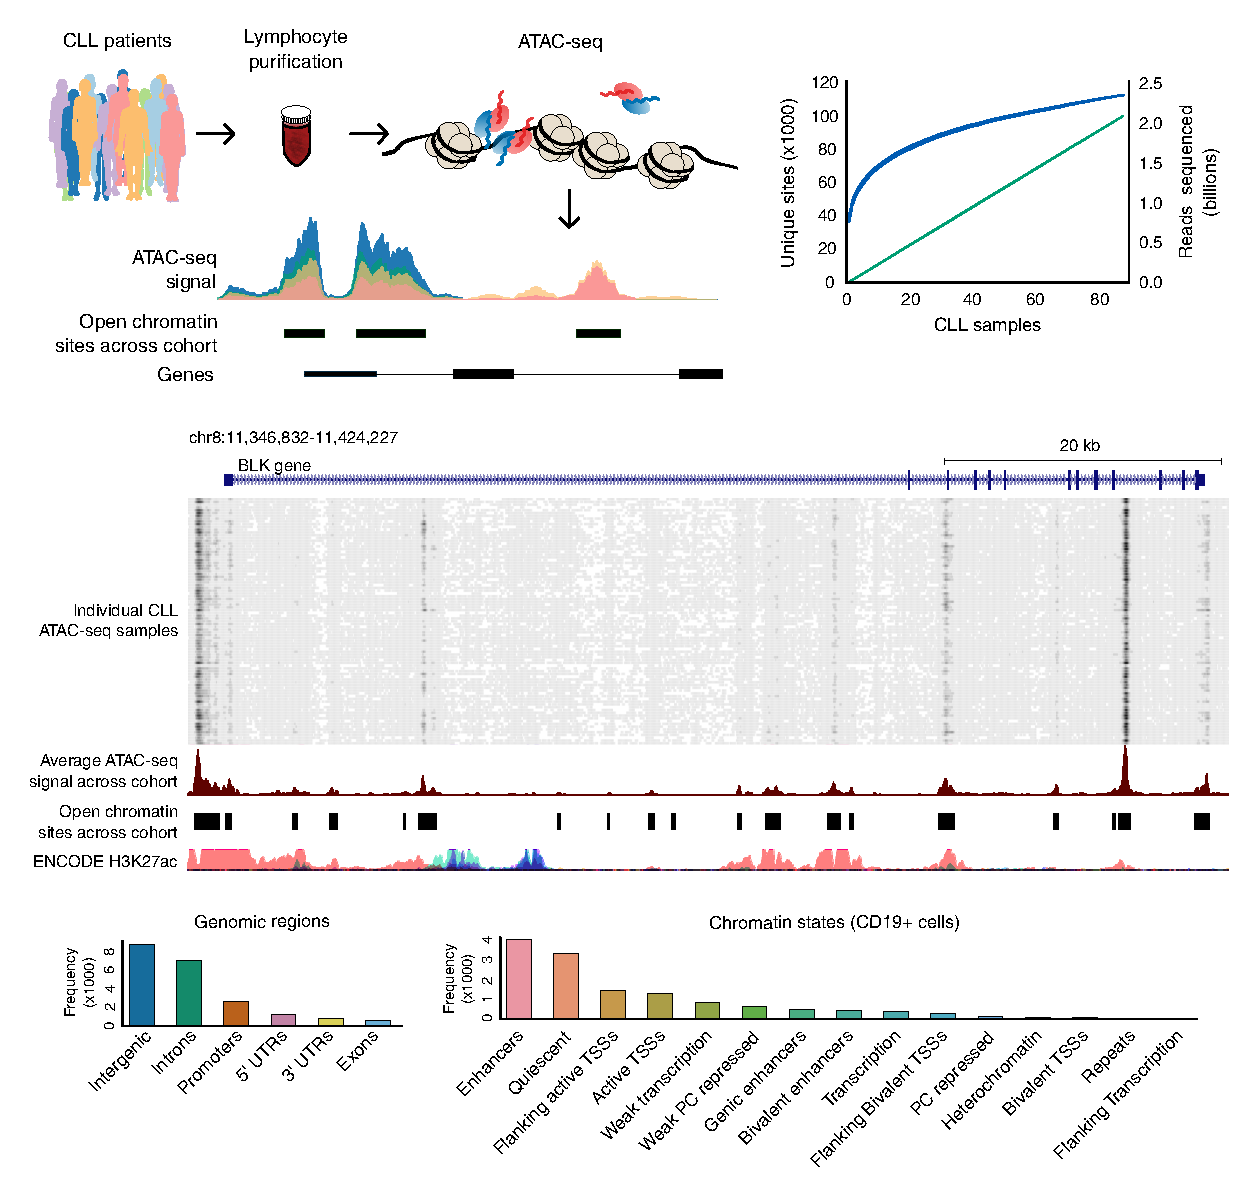
\includegraphics[width=1.000\hsize]{figures/Figure1.pdf}
\caption{\emph{The chromatin accessibility landscape of chronic
lymphocytic leukemia (CLL).} \textbf{a)} ATAC-seq profiling and analysis
workflow for establishing patient-specific and cohort-level maps of
chromatin accessibility in CLL. \textbf{b)} Saturation analysis showing
the number of unique chromatin-accessible regions detected across 88
samples and with a total sequencing depth of 2.2 billion ATAC-seq
fragments. The narrow blue and green corridors indicate 95\% confidence
intervals for samples added in random order (1,000 iterations).
\textbf{c)} Genome browser plot showing ATAC-seq signal intensity for 88
individual CLL samples (top), average signal intensity across the cohort
and cohort-level peak calls (center), and reference data from the ENCODE
project (bottom). Interactive genome browser tracks are available from
the supplementary website:
\url{http://cll-chromatin.computational-epigenetics.org/}. \textbf{d)}
Absolute (frequency) and relative (fold-change) co-localization of
unique chromatin-accessible regions in CLL with gene annotations (left)
and chromatin state segmentations for CD19+ B cells from the Roadmap
Epigenomics project (right).}\label{Figure1}
\end{figure}

\begin{figure}
\centering
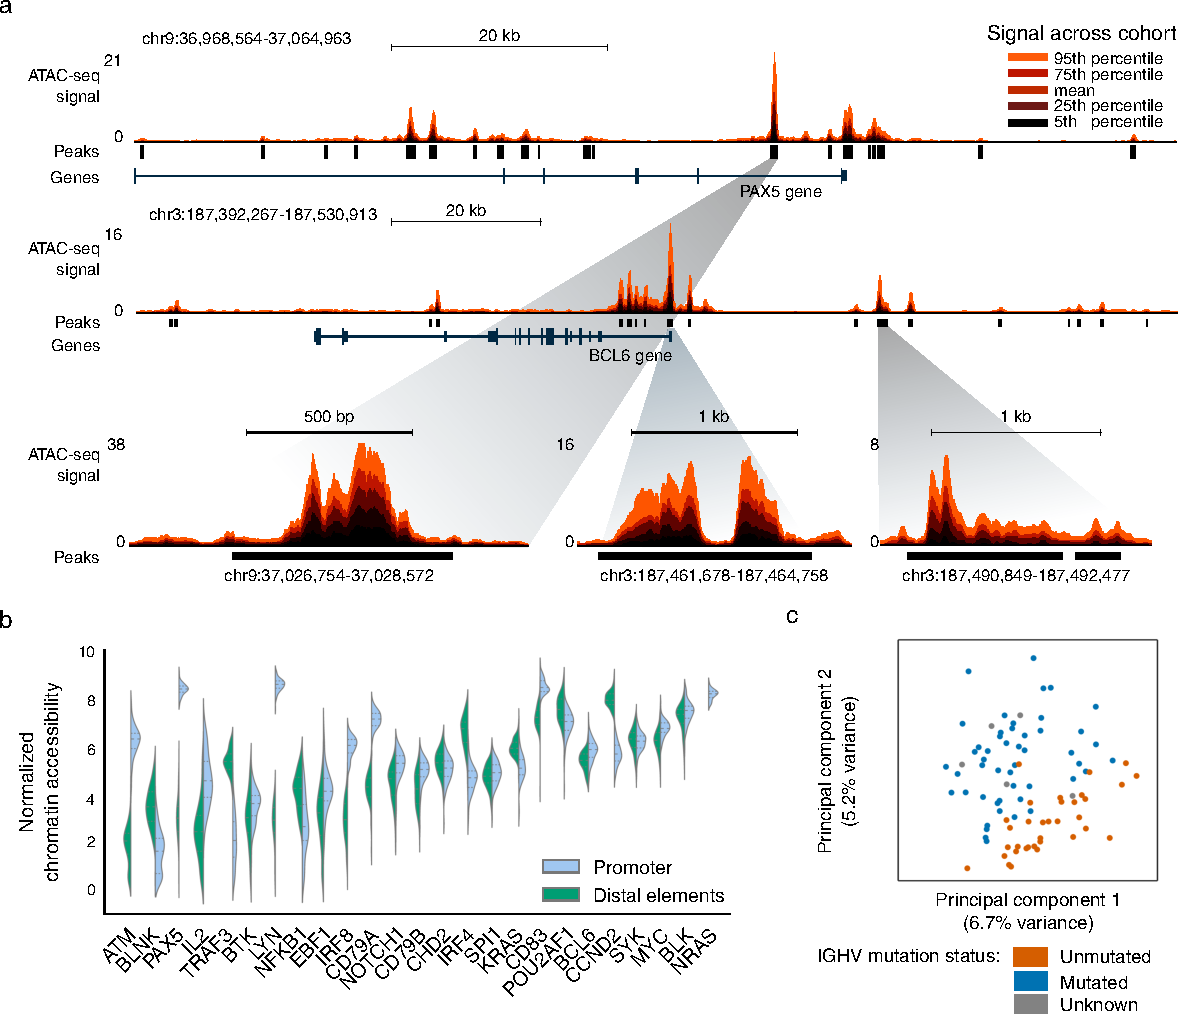
\includegraphics[width=1.000\hsize]{figures/Figure2.pdf}
\caption{\emph{Heterogeneity in the CLL chromatin accessibility
landscape.} \textbf{a)} Genome browser plot showing ATAC-seq signal
intensity across the CLL cohort in the vicinity of two genes with a
known role in B cell biology (PAX5 and BCL6). This cohort-level track
uses color-coded percentiles to visualize the observed heterogeneity
between samples. The bottom row zooms in on the chromatin accessibility
landscape at three specific regulatory regions. \textbf{b)} Violin plots
showing the cohort-wide distribution of chromatin accessibility at
promoters (chromatin-accessible regions located with 2,500 basepairs
from the transcription start site) and putative enhancers of genes with
a known role in B cell biology and/or CLL pathogenesis. \textbf{c)}
Unsupervised principal component analysis based on the chromatin
accessibility for all 88 samples at each of the 112,298
chromatin-accessible regions in the CLL cohort. Samples are color-coded
according to their IGHV mutation status, using \textless{} 98\% germline
homology as threshold for classifying a sample as
mutated.}\label{Figure2}
\end{figure}

\begin{figure}
\centering
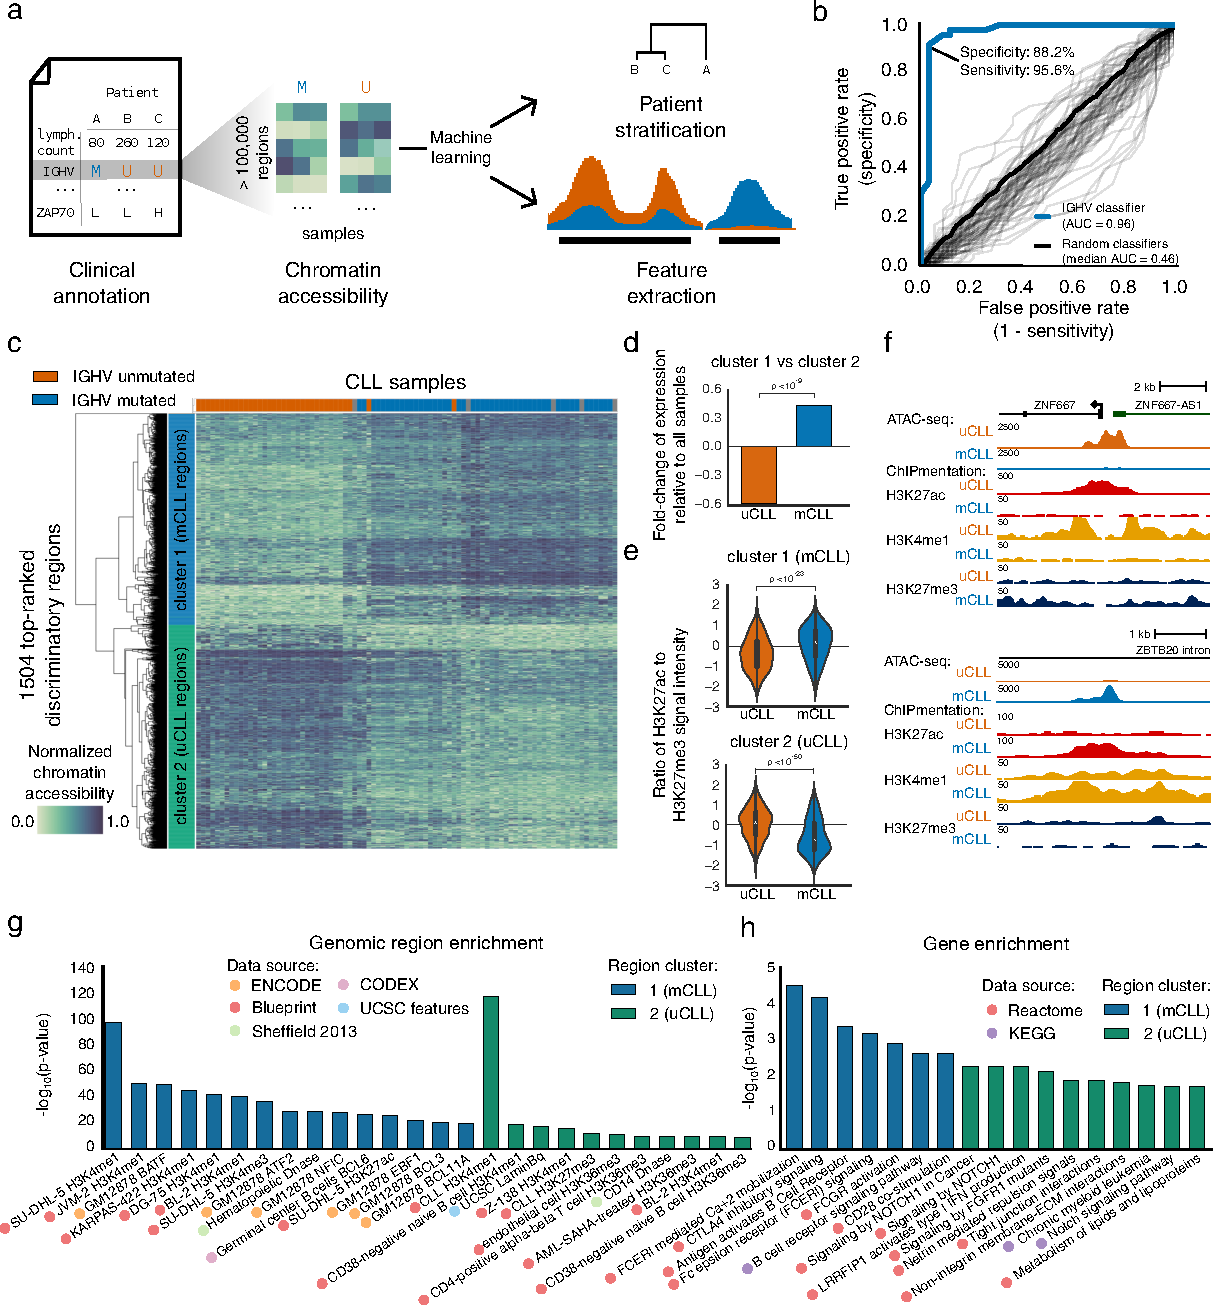
\includegraphics[width=0.850\hsize]{figures/Figure3.pdf}
\caption{\emph{Disease subtype-specific patterns of chromatin
accessibility.} \textbf{a)} Methodology for deriving disease
subtype-specific patterns of chromatin accessibility: A machine learning
algorithm is trained to distinguish between different sample sets (here:
IGHV-mutated vs.~IGHV-unmutated), the prediction performance is
evaluated by cross-validation, and the most predictive features are
obtained by feature extraction from the trained classifiers. \textbf{b)}
ROC curve summarizing the test set prediction performance (estimated by
leave-one-out cross-validation) of a random forest classifier that uses
the ATAC-seq dataset to distinguish between IGHV-mutated and
IGHV-unmutated samples. ``AUC'' refers to the ROC area under curve as a
measure of prediction performance, and sensitivity/specificity values
are shown for the point on the ROC curve that is closest to the top left
corner. The grey lines indicate the performance of 1,000 classifiers
trained and evaluated in the same way but based on randomly shuffled
class labels. \textbf{c)} Clustered heatmap based on the most predictive
regions extracted from the cross-validated classifiers. \textbf{d)}
Ratio of expression levels for genes linked to mCLL-accessible regions
vs.~genes linked to uCLL-accessible regions. \textbf{e)} Ratio between
ChIPmentation signal for active chromatin (H3K27ac) and repressive
chromatin (H3K27me3) at mCLL-linked and uCLL-linked regions. \textbf{f)}
Genome browser plots showing ATAC-seq and ChIPmentation profiles for
gene loci with a known role in CLL (ZNF667 and ZBTB20). \textbf{g)} Most
highly enriched region sets for mCLL (blue) and uCLL (green) associated
regions. \textbf{h)} Most highly enriched pathways among genes linked to
mCLL (blue) and uCLL (green) regions.}\label{Figure3}
\end{figure}

\begin{figure}
\centering
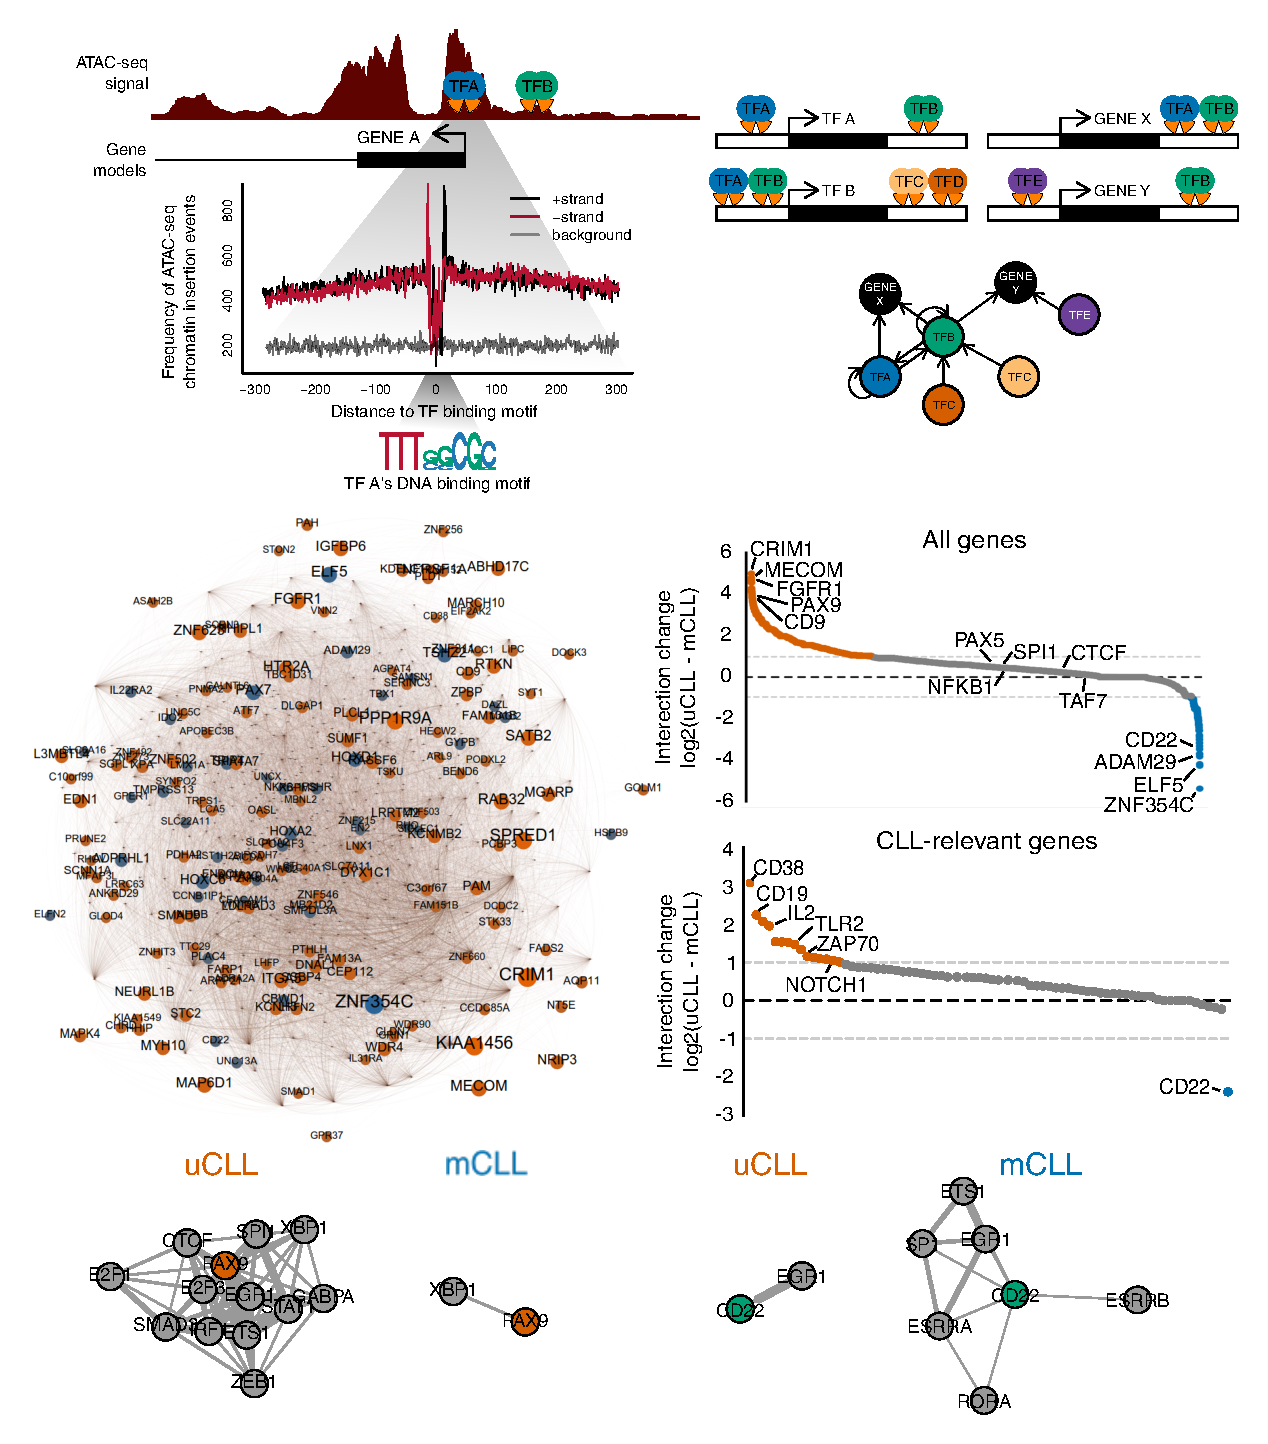
\includegraphics[width=1.000\hsize]{figures/Figure4.pdf}
\caption{\emph{Patient stratification into CLL subtypes based on
chromatin accessibility.} \textbf{a)} Hierarchical clustering of all CLL
samples based the classifiers' most predictive regions. Clusters 1
corresponds to mCLL, cluster 4 to uCLL, and the clusters 2 and 3
correspond to iCLL. Samples are colored by IGHV mutation status (top)
and cluster assignment (bottom). \textbf{b)} Principal component
analysis for the same data as in panel a, showing the first two
principal components as well as their explained
variance.}\label{Figure4}
\end{figure}

\begin{figure}
\centering
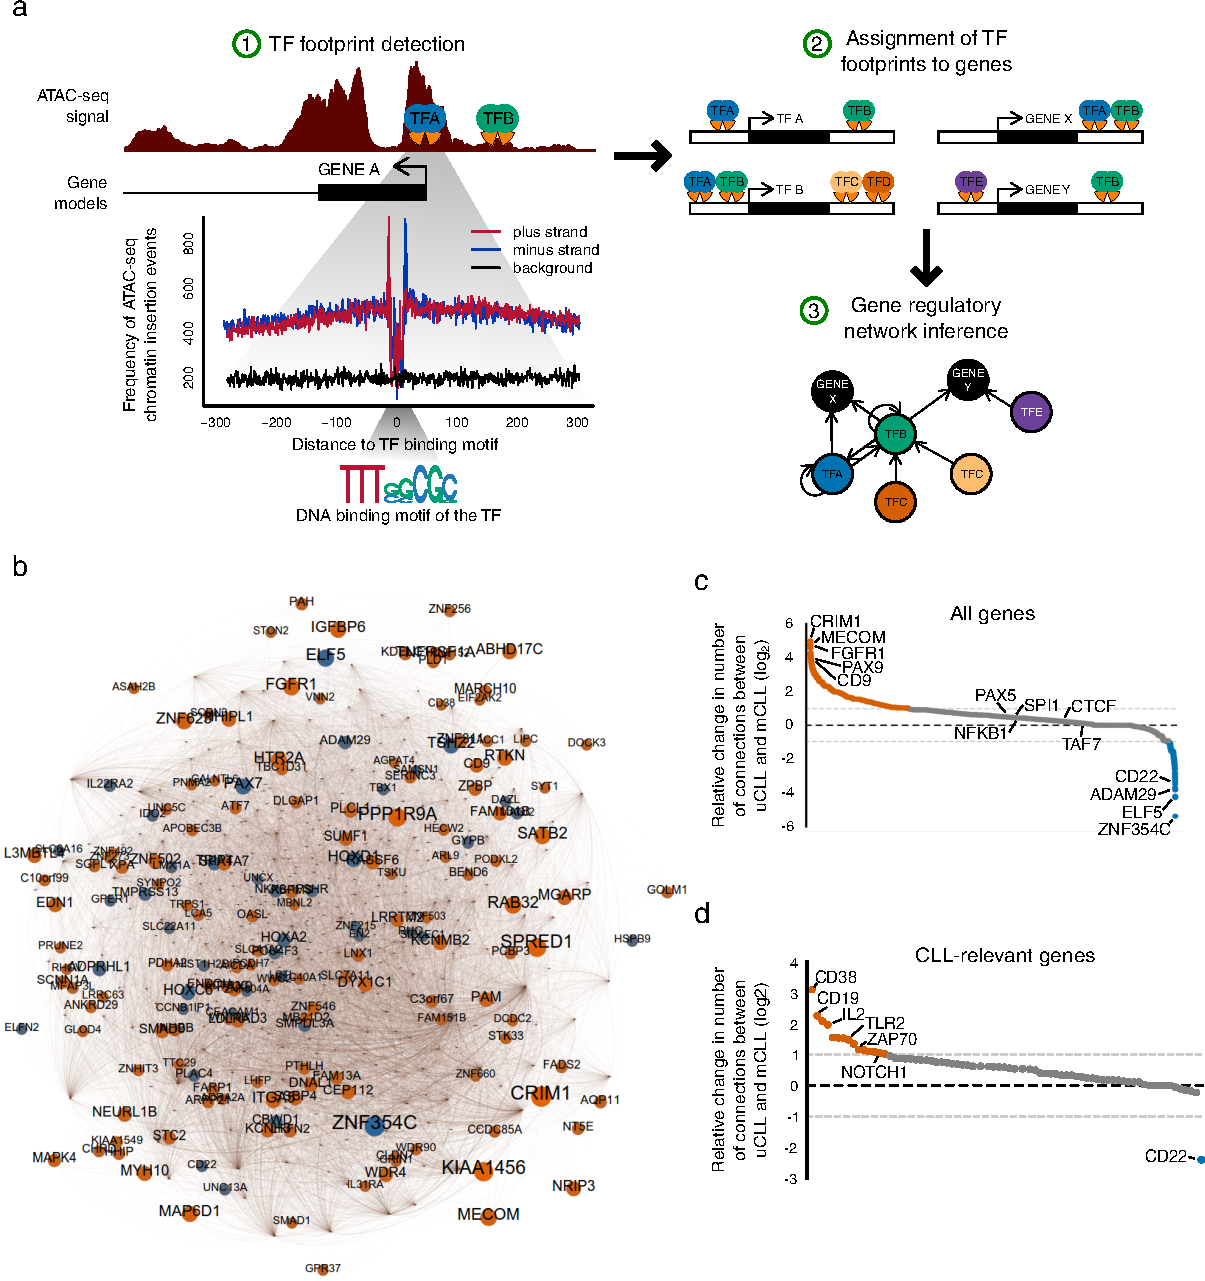
\includegraphics[width=1.000\hsize]{figures/Figure5.pdf}
\caption{\emph{Gene regulatory networks underlying the mCLL and uCLL
disease subtypes.} \textbf{a)} Methodology for deriving gene regulatory
networks from ATAC-seq data using transcription factor (TF)
footprinting, mapping of transcription factor binding footprints to
co-localized genes, and regulatory network inference. \textbf{b)} CLL
gene regulatory network derived from the data of all 88 samples, showing
the most differentially connected genes between uCLL and mCLL (the full
network is shown in Supplementary Figure 18). Node size reflects the
total number of connections of each node, and colors denote the
subtype-specific network in which the nodes are more highly connected
(mCLL: blue; uCLL: orange). \textbf{c)} Relative change in the number of
connections between the mCLL and uCLL networks, showing all genes.
\textbf{d)} Relative change in the number of connections between the
mCLL and uCLL networks, focusing on genes with a known role in B cell
biology and/or CLL pathogenesis.}\label{Figure5}
\end{figure}
\clearpage

\section{Supplemental Data}\label{supplemental-data}

\subsection{Supplementary Data 1: Clinical annotations of the CLL
patient
cohort.}\label{supplementary-data-1-clinical-annotations-of-the-cll-patient-cohort.}

Clinical annotations for the patient samples that were analyzed in this
study. All patients were diagnosed and treated at the Royal Bournemouth
Hospital (UK).

\subsection{Supplementary Data 2: Summary statistics of the sequencing
experiments.}\label{supplementary-data-2-summary-statistics-of-the-sequencing-experiments.}

Sequencing statistics for 88 samples with ATAC-seq, 10 samples with
ChIPmentation for three histone marks (H3K4me1, H3K27ac, H3K27me3) and
one control (IgG), and 10 samples with RNA-seq.

\subsection{Supplementary Data 3: Differentially expressed genes between
CLL
subtypes.}\label{supplementary-data-3-differentially-expressed-genes-between-cll-subtypes.}

List of differentially expressed genes between three disease subtypes
(mCLL, iCLL, uCLL), based on RNA-seq data for representative samples in
each subtype.

\subsection{Supplementary Data 4: Chromatin-accessible regions
associated with IGHV mutation
status.}\label{supplementary-data-4-chromatin-accessible-regions-associated-with-ighv-mutation-status.}

List of regions with differential chromatin accessibility between
IGHV-mutated and IGHV-unmutated CLL samples, based on the machine
learning analysis or alternatively based on differential peak analysis
using DESeq2.

\begin{figure}
\centering
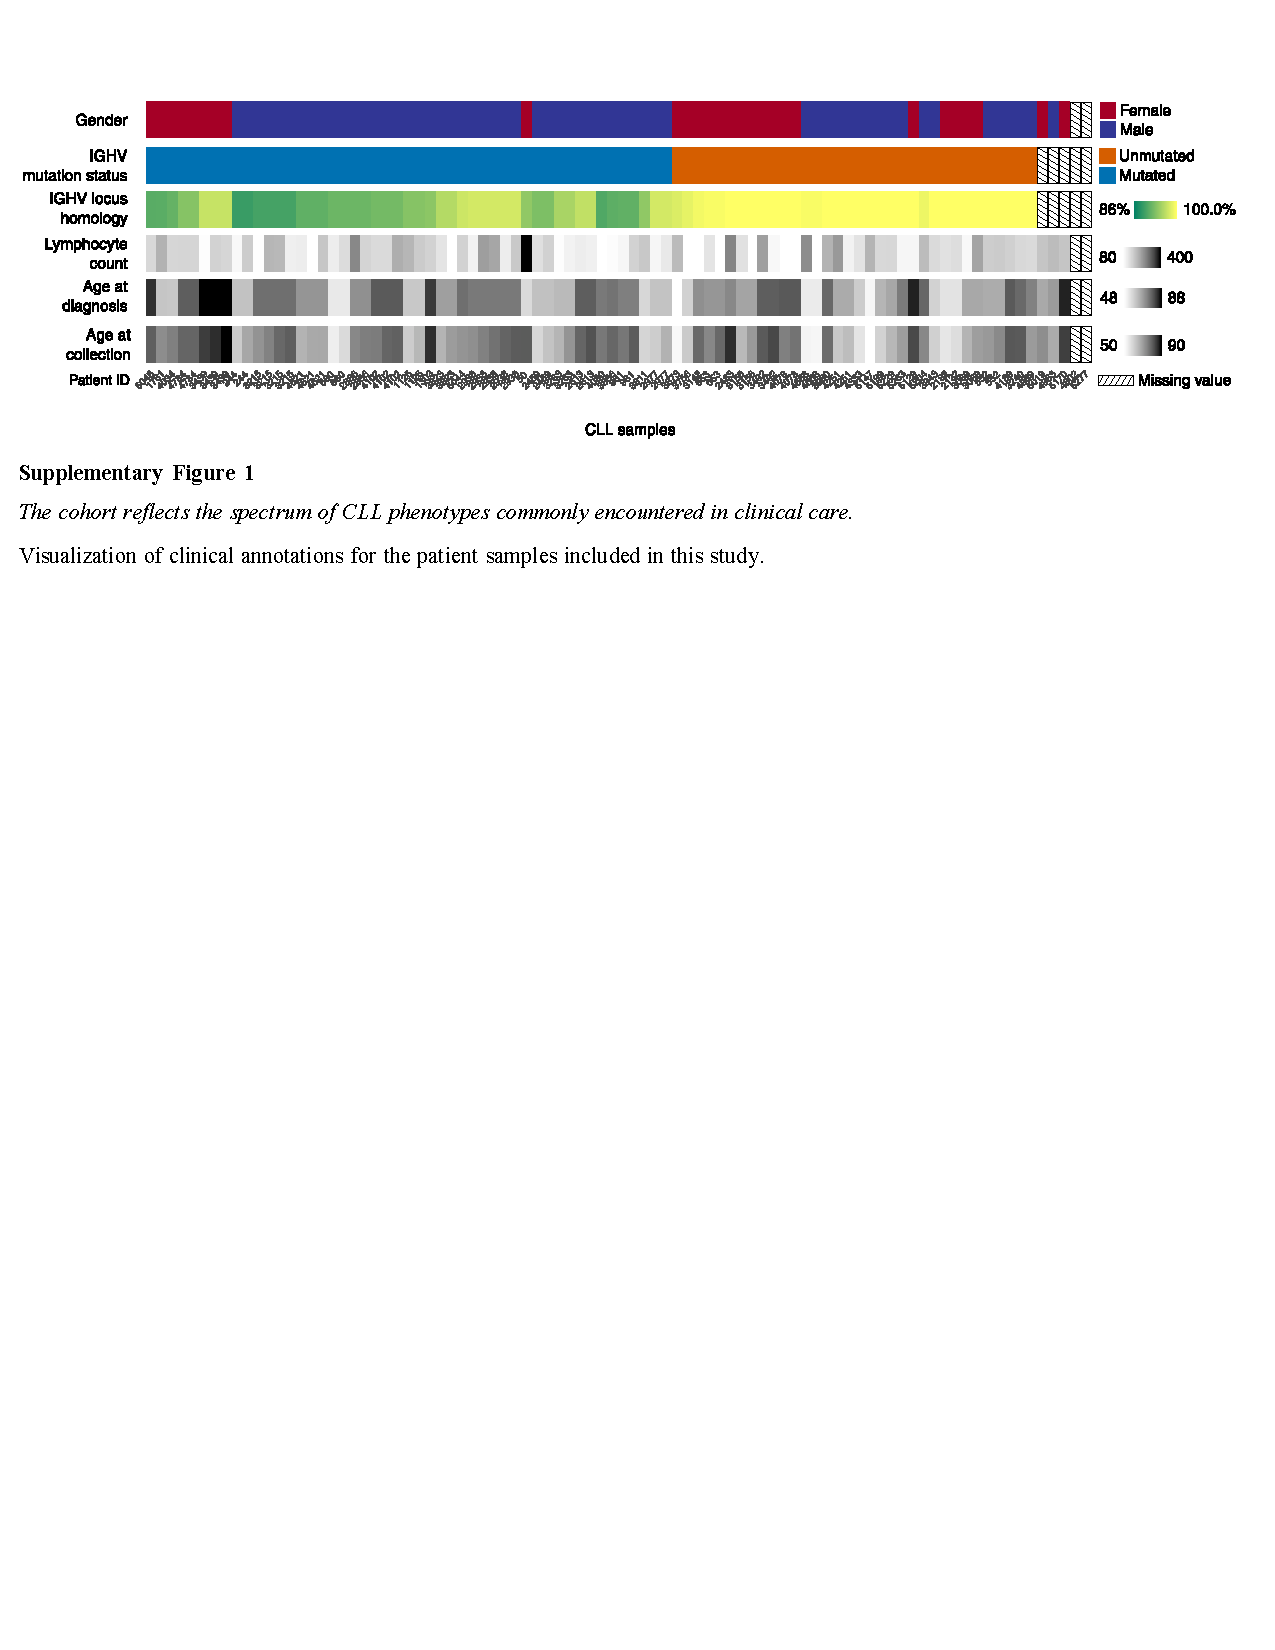
\includegraphics[width=1.000\hsize]{figures/Supplementary_Information_01.pdf}
\end{figure}
\clearpage

\begin{figure}
\centering
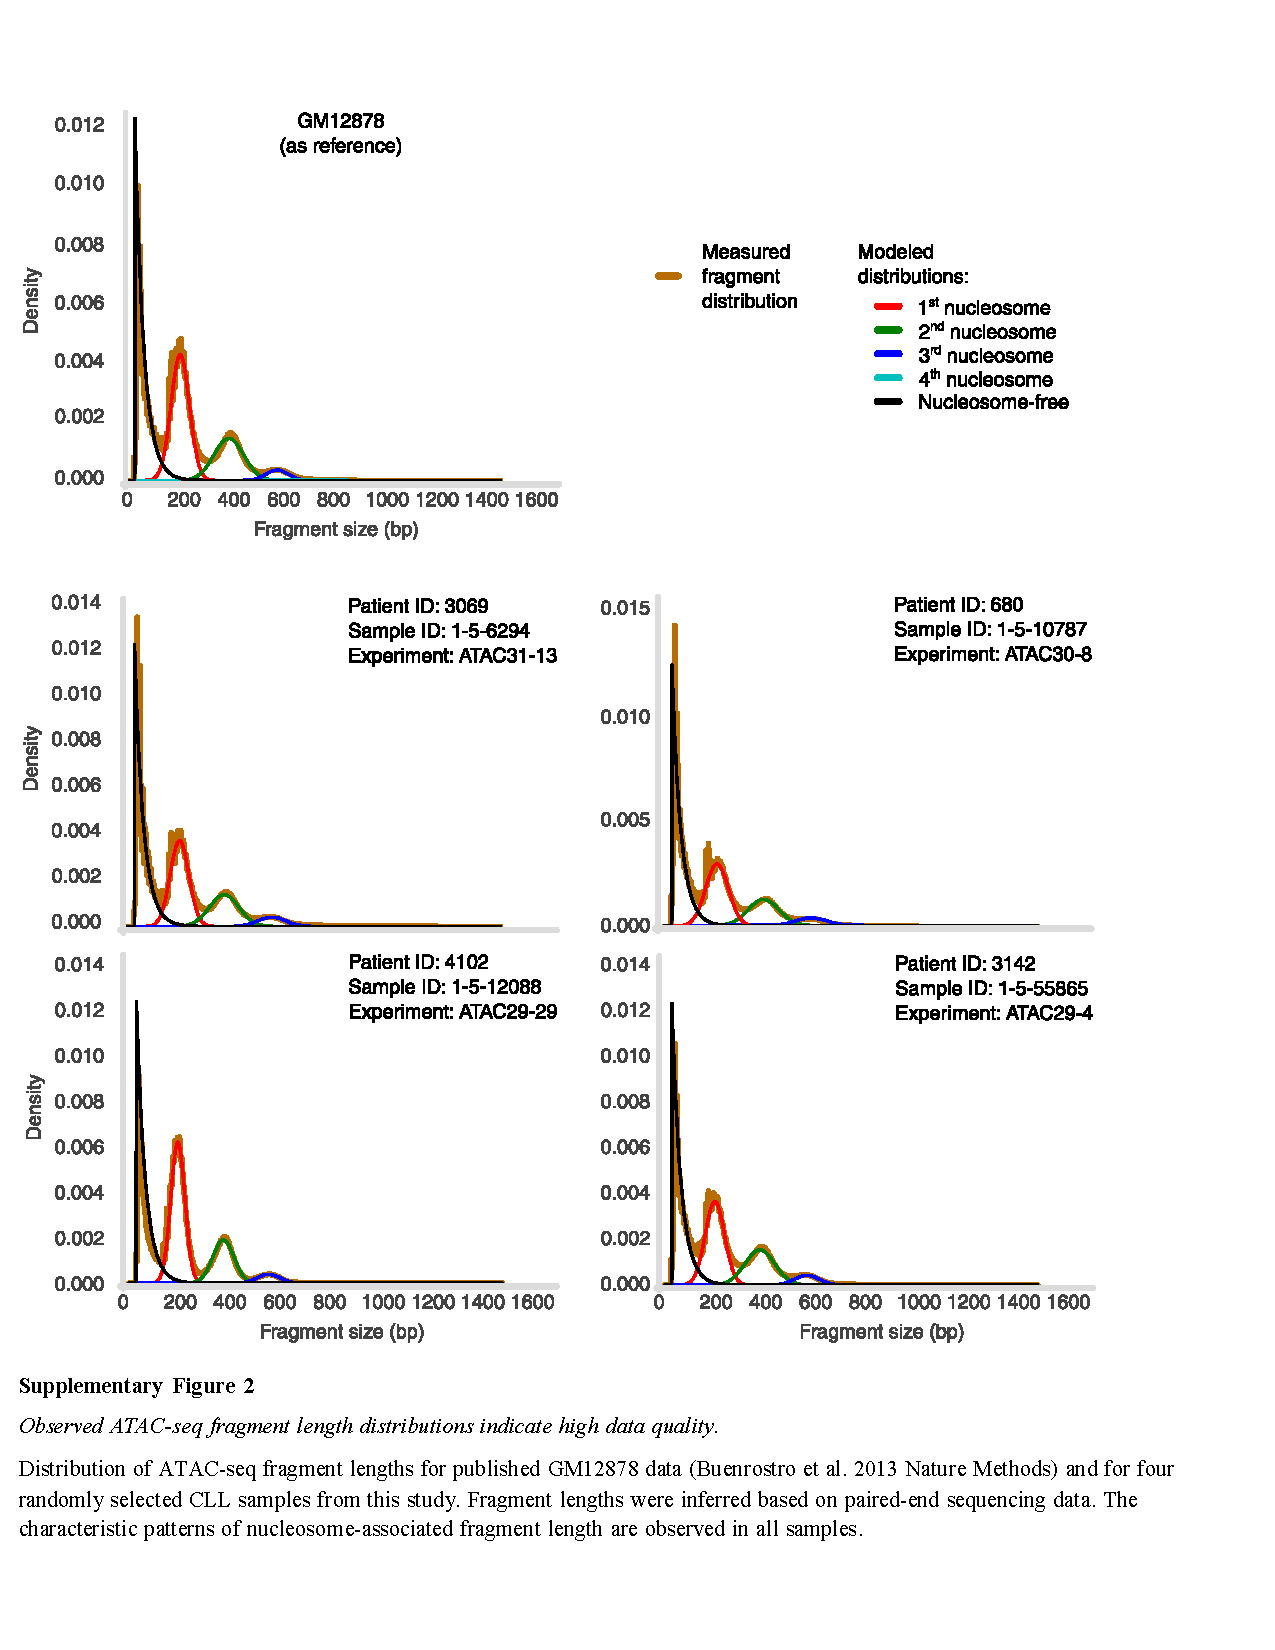
\includegraphics[width=1.000\hsize]{figures/Supplementary_Information_02.pdf}
\end{figure}
\clearpage

\begin{figure}
\centering
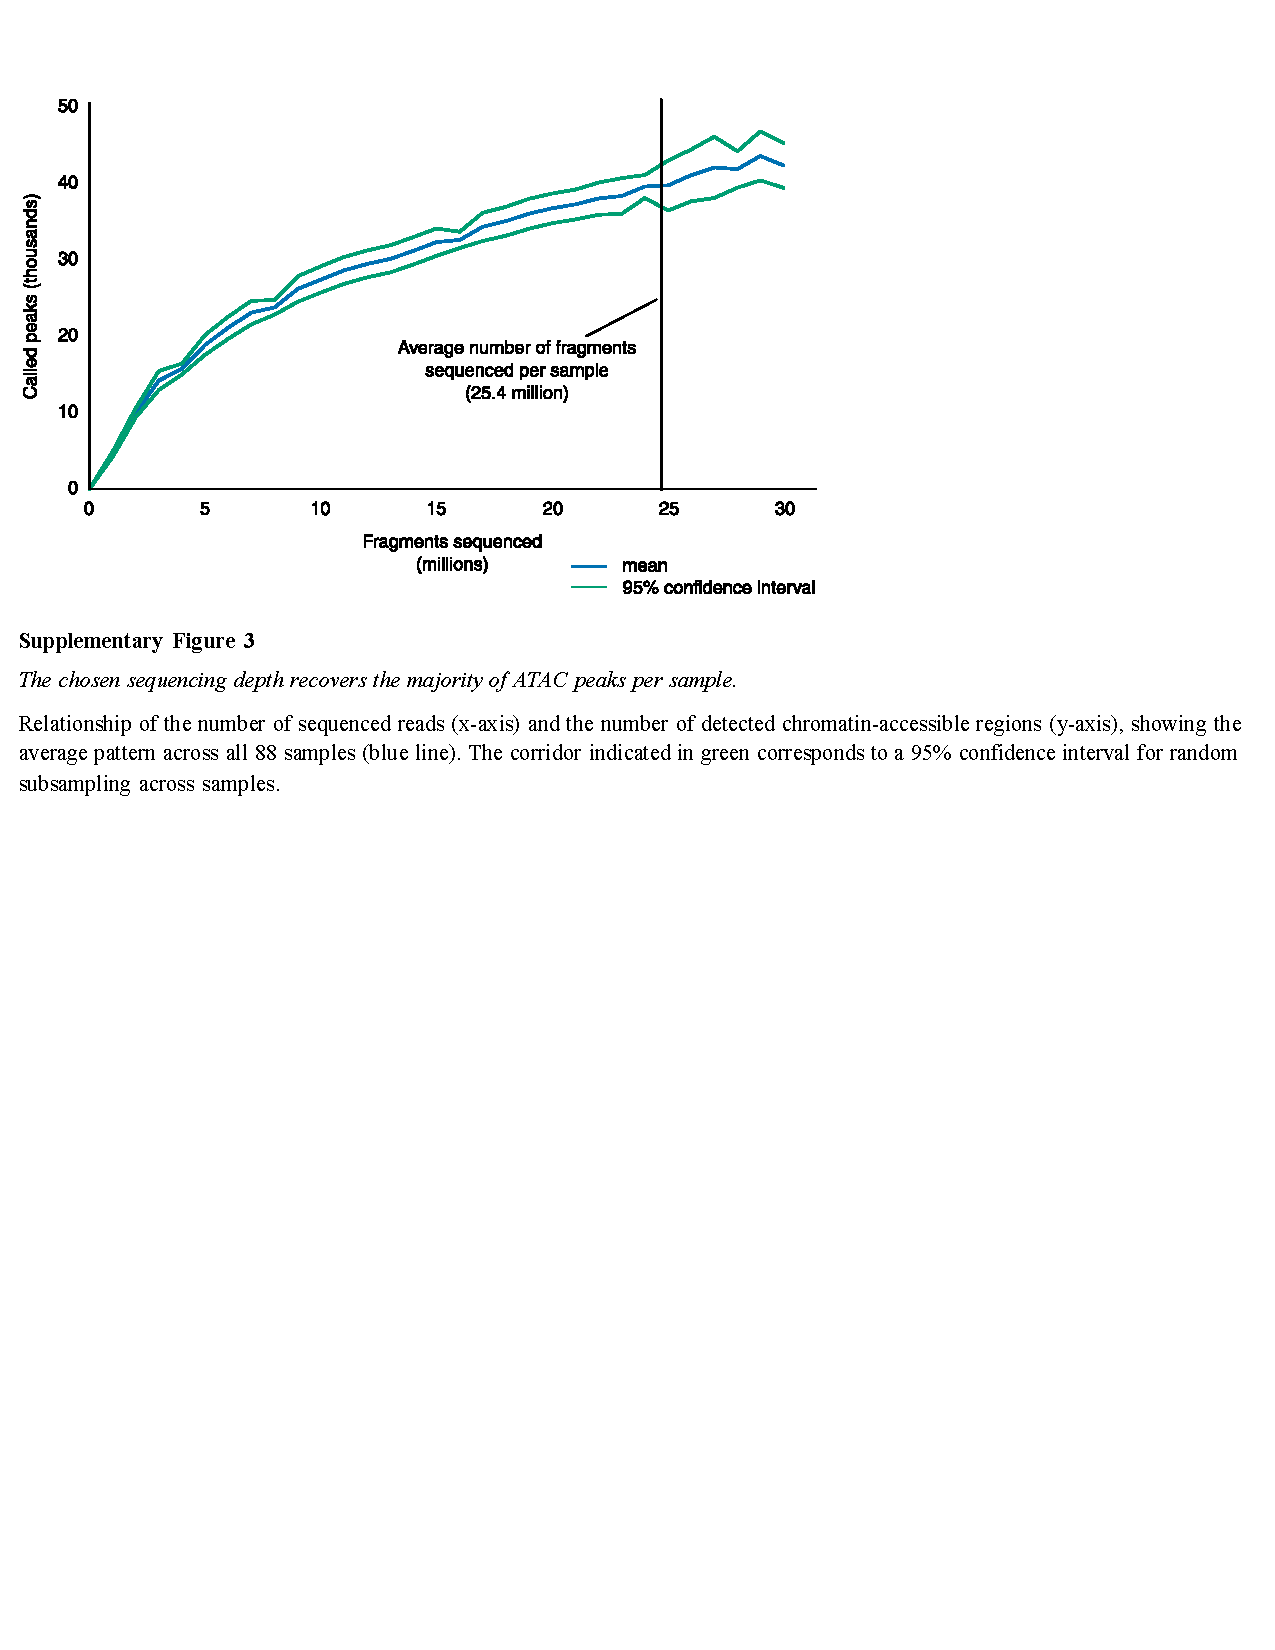
\includegraphics[width=1.000\hsize]{figures/Supplementary_Information_03.pdf}
\end{figure}
\clearpage

\begin{figure}
\centering
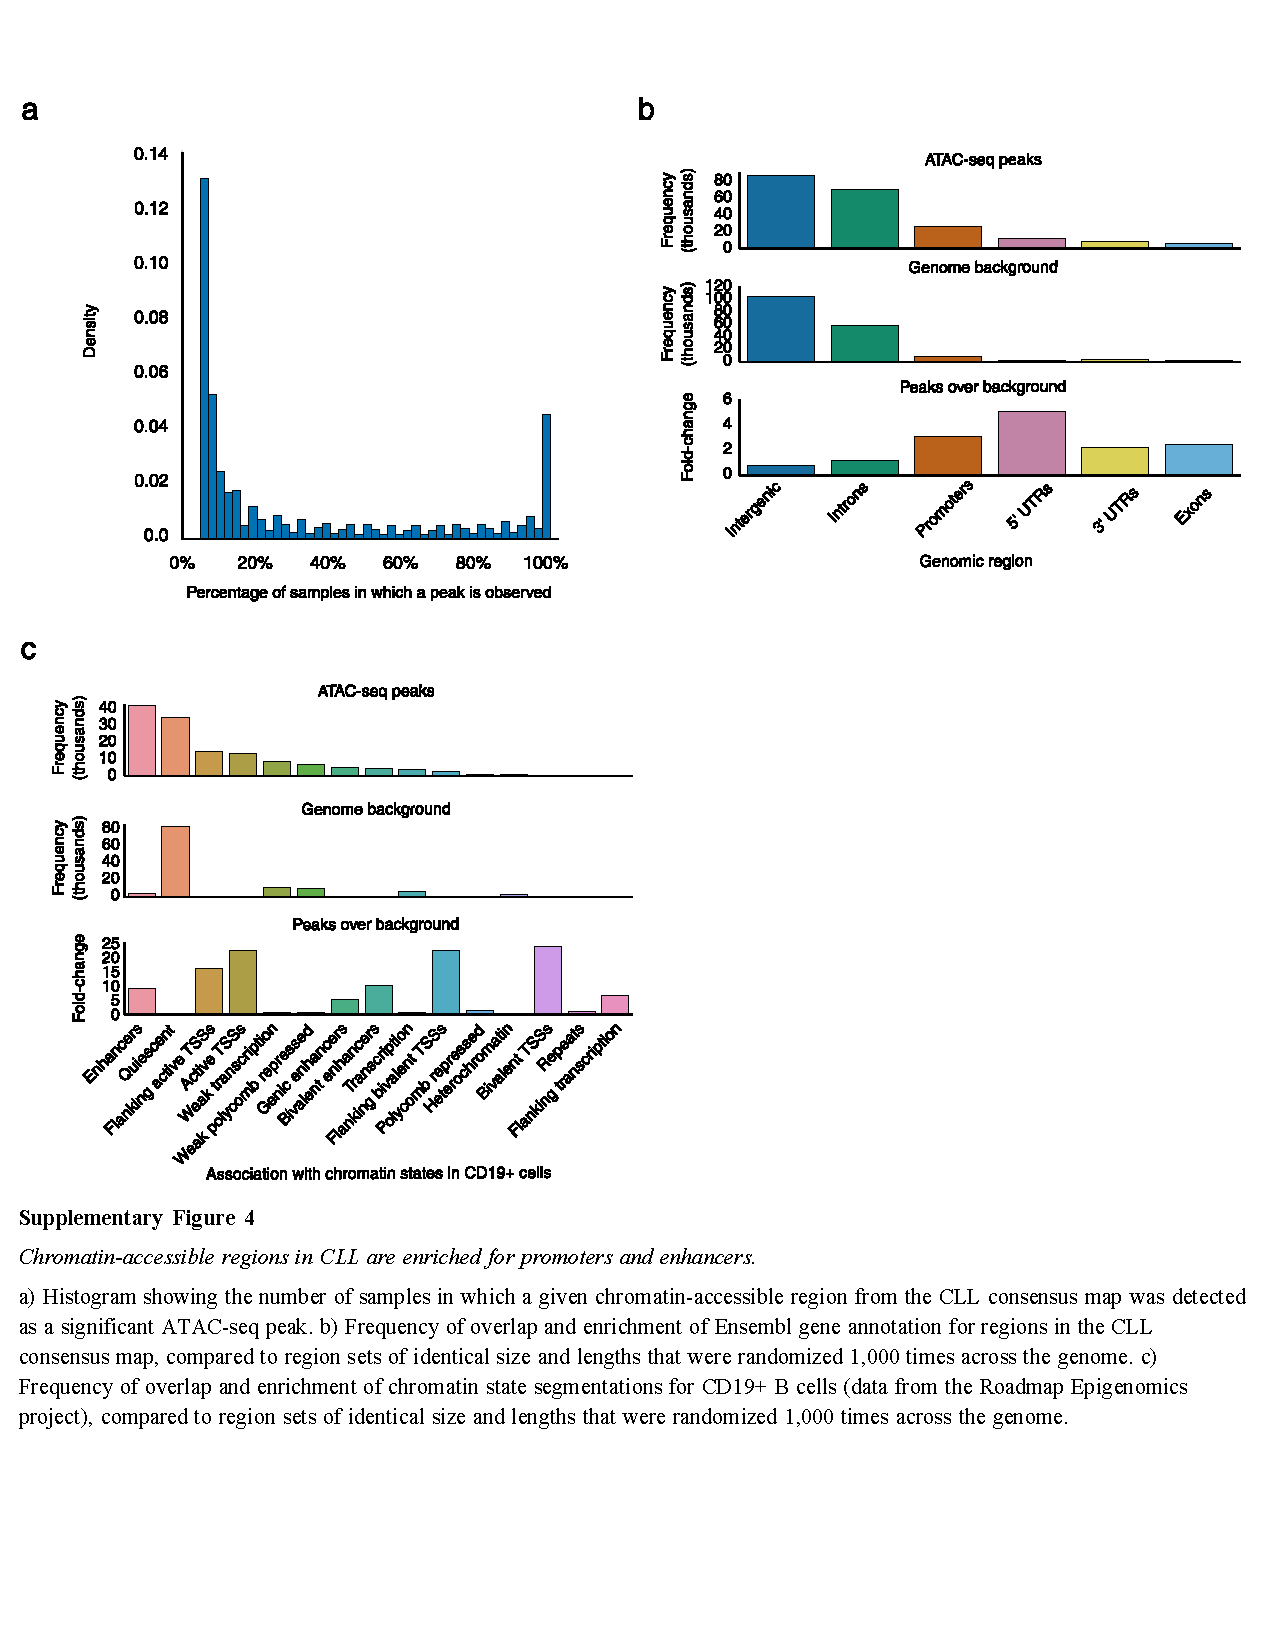
\includegraphics[width=1.000\hsize]{figures/Supplementary_Information_04.pdf}
\end{figure}
\clearpage

\begin{figure}
\centering
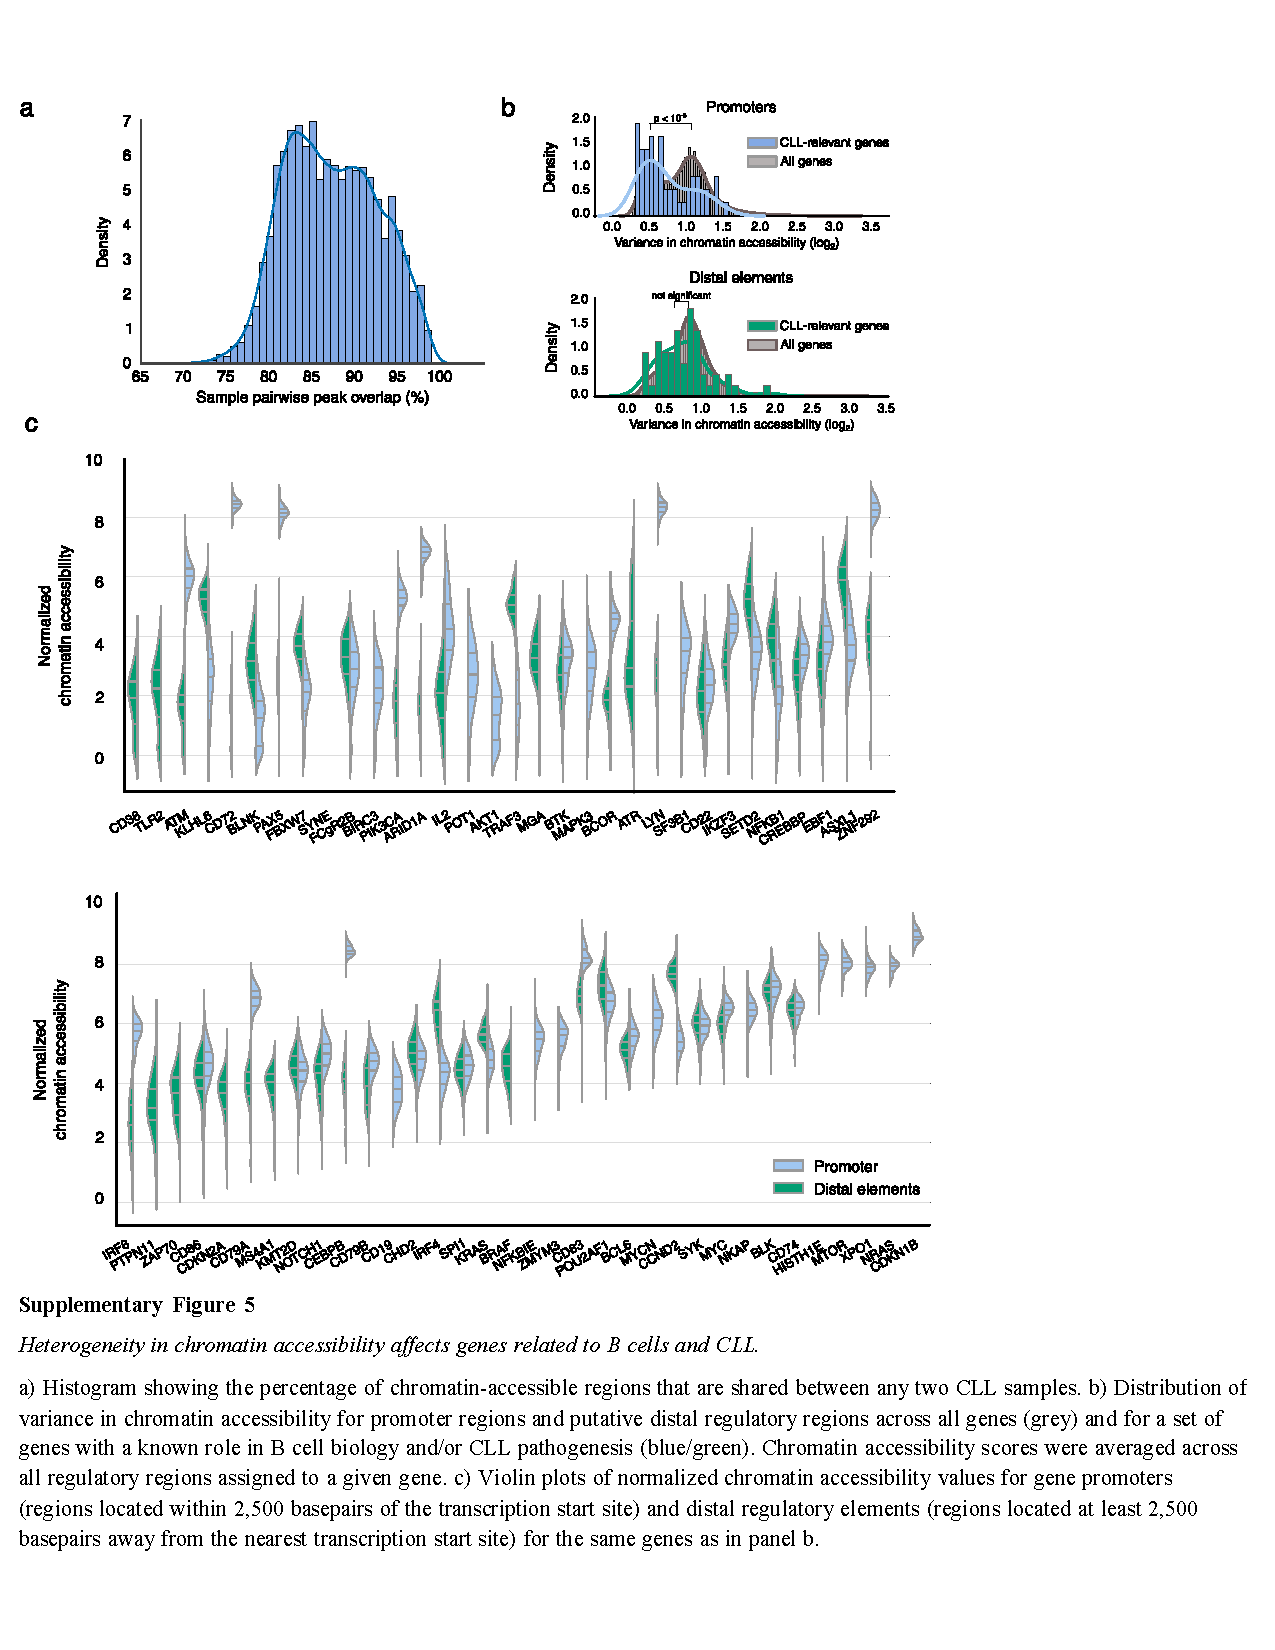
\includegraphics[width=1.000\hsize]{figures/Supplementary_Information_05.pdf}
\end{figure}
\clearpage

\begin{figure}
\centering
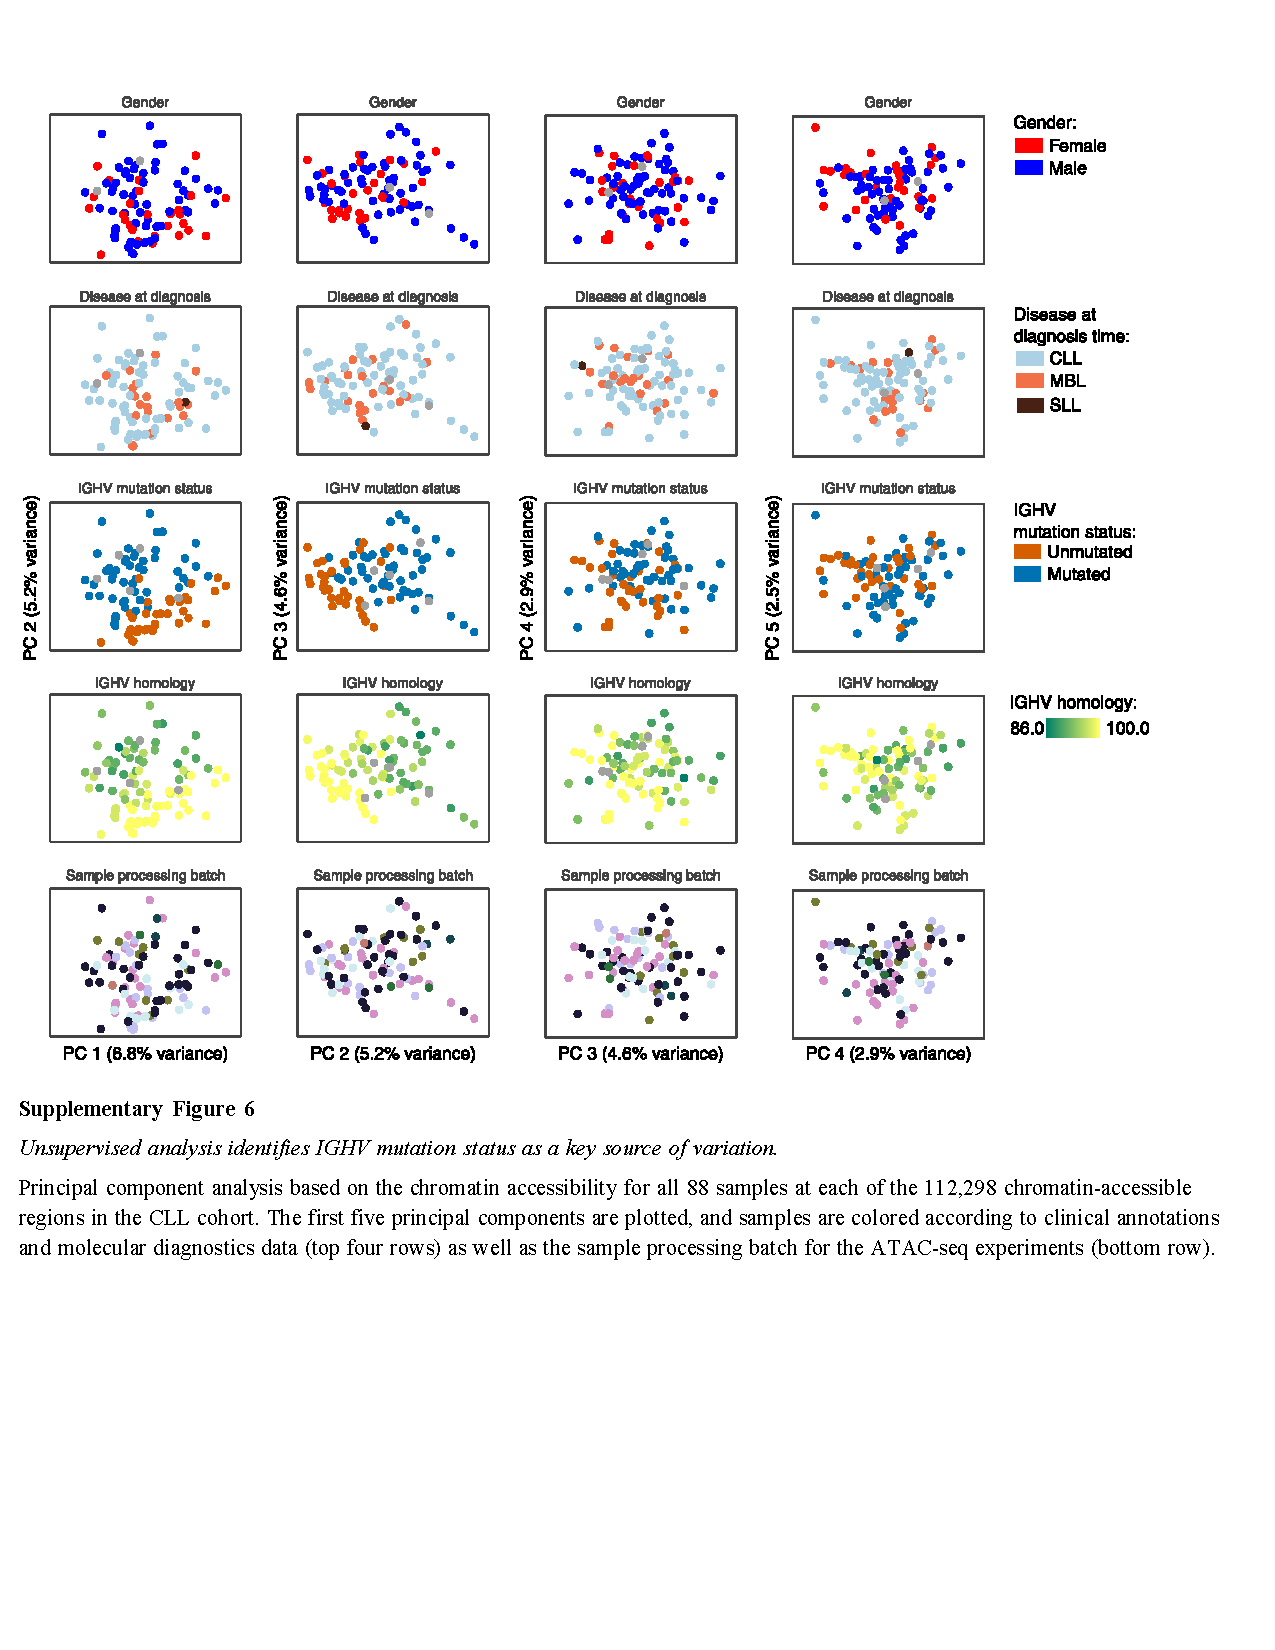
\includegraphics[width=1.000\hsize]{figures/Supplementary_Information_06.pdf}
\end{figure}
\clearpage

\begin{figure}
\centering
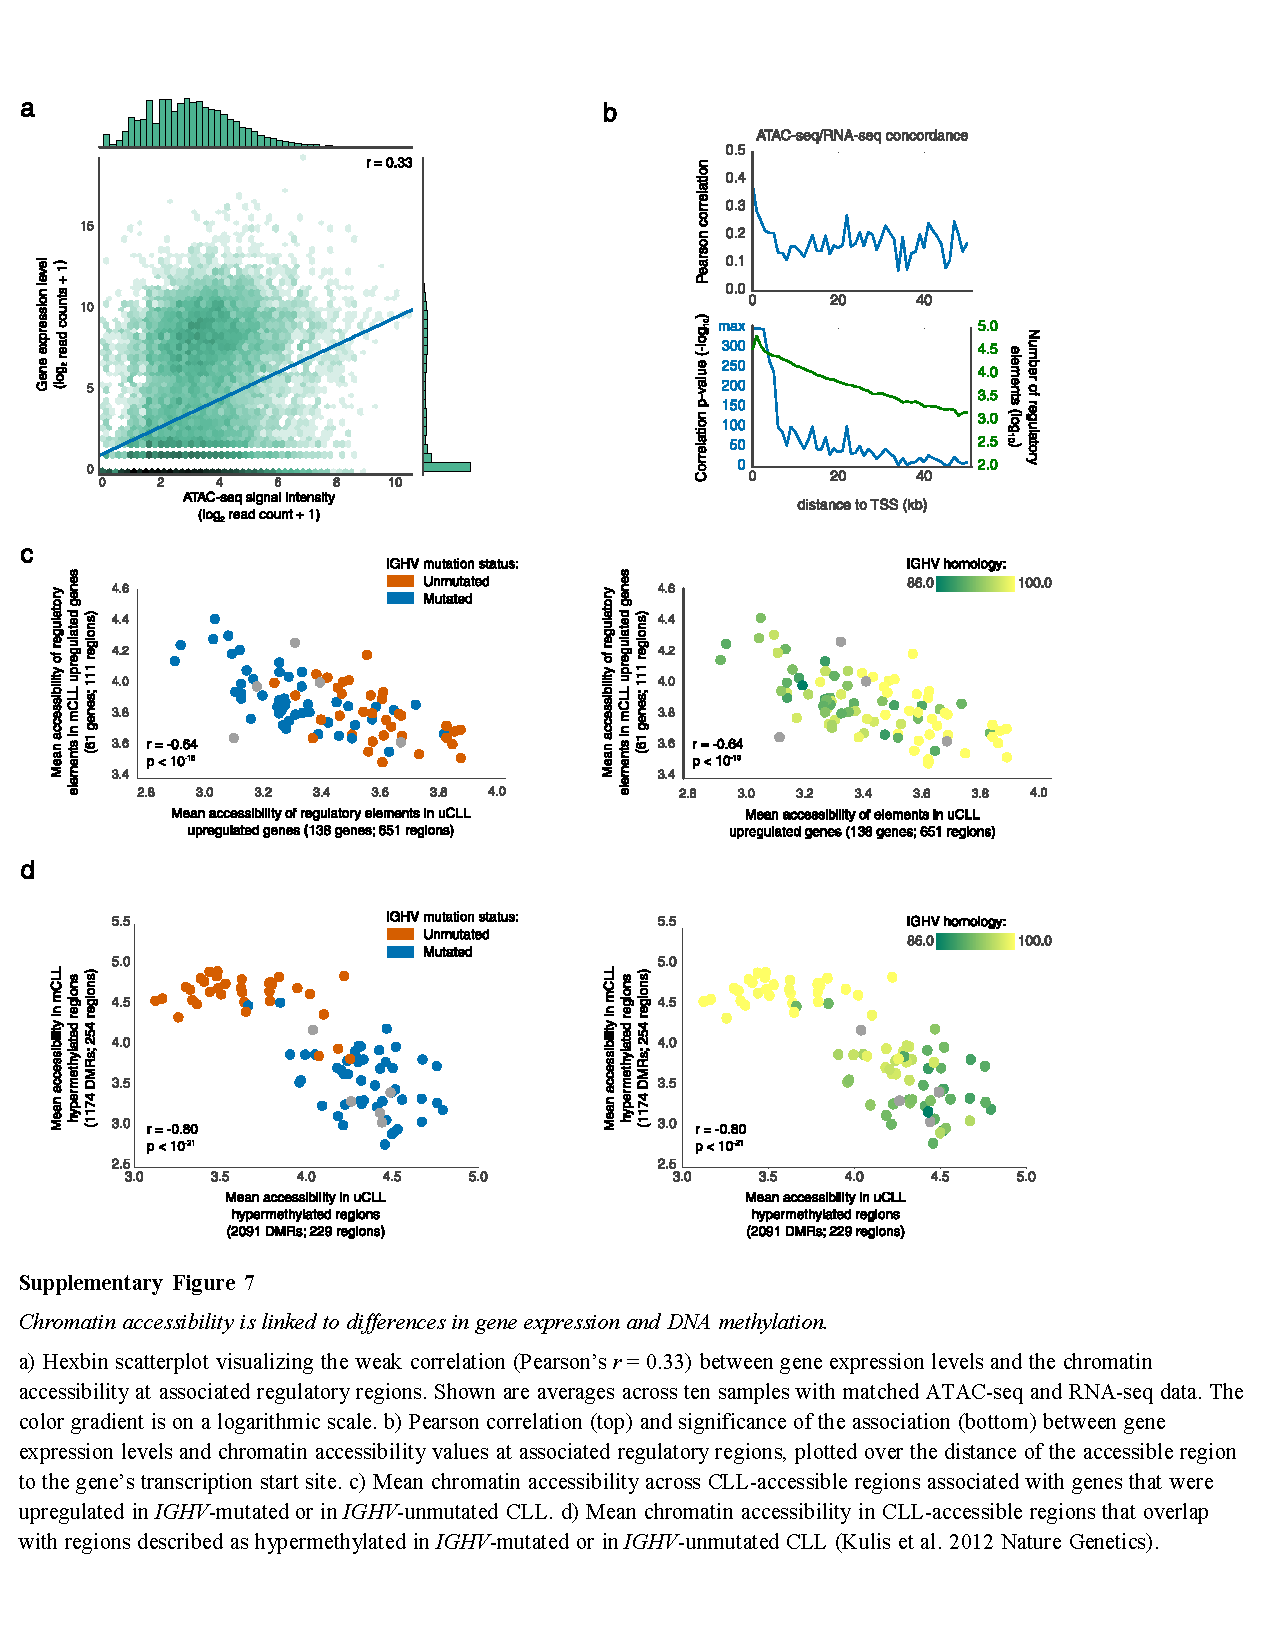
\includegraphics[width=1.000\hsize]{figures/Supplementary_Information_07.pdf}
\end{figure}
\clearpage

\begin{figure}
\centering
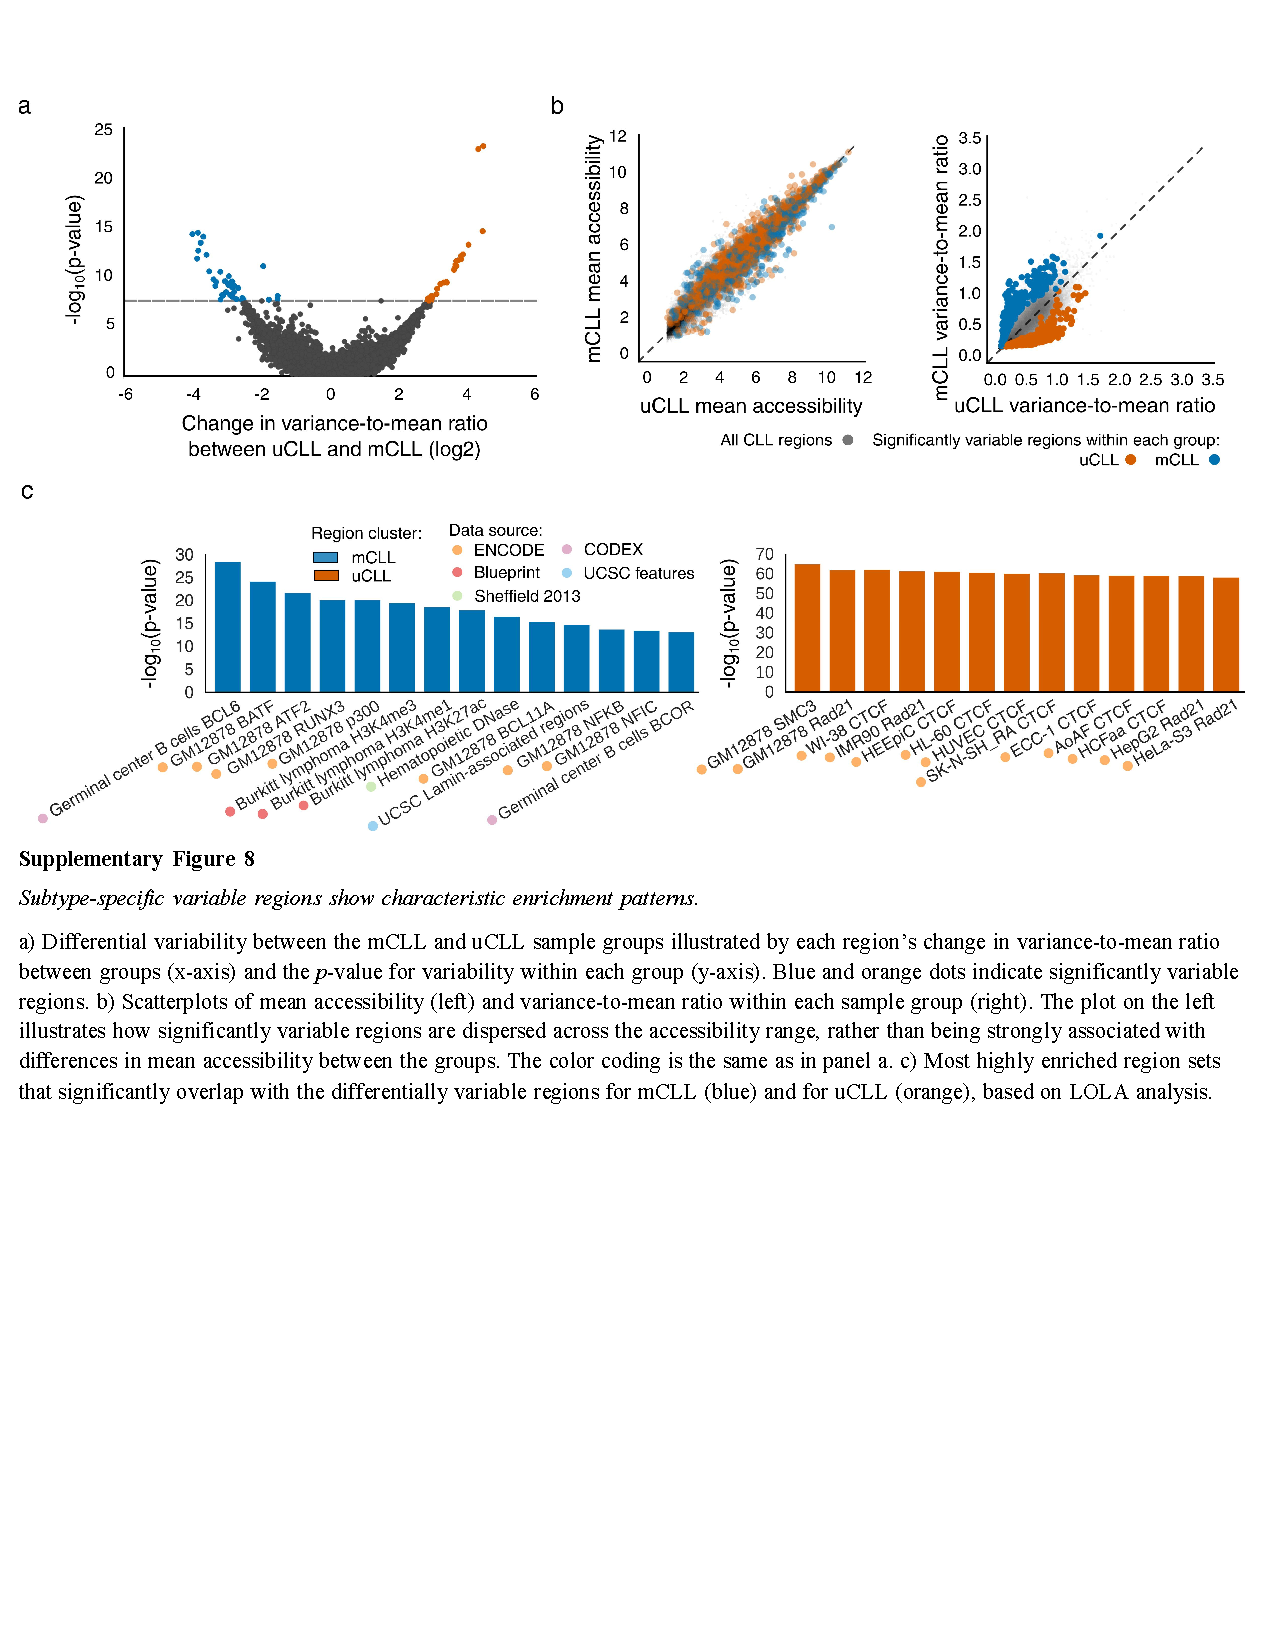
\includegraphics[width=0.900\hsize]{figures/Supplementary_Information_08.pdf}
\end{figure}
\clearpage

\begin{figure}
\centering
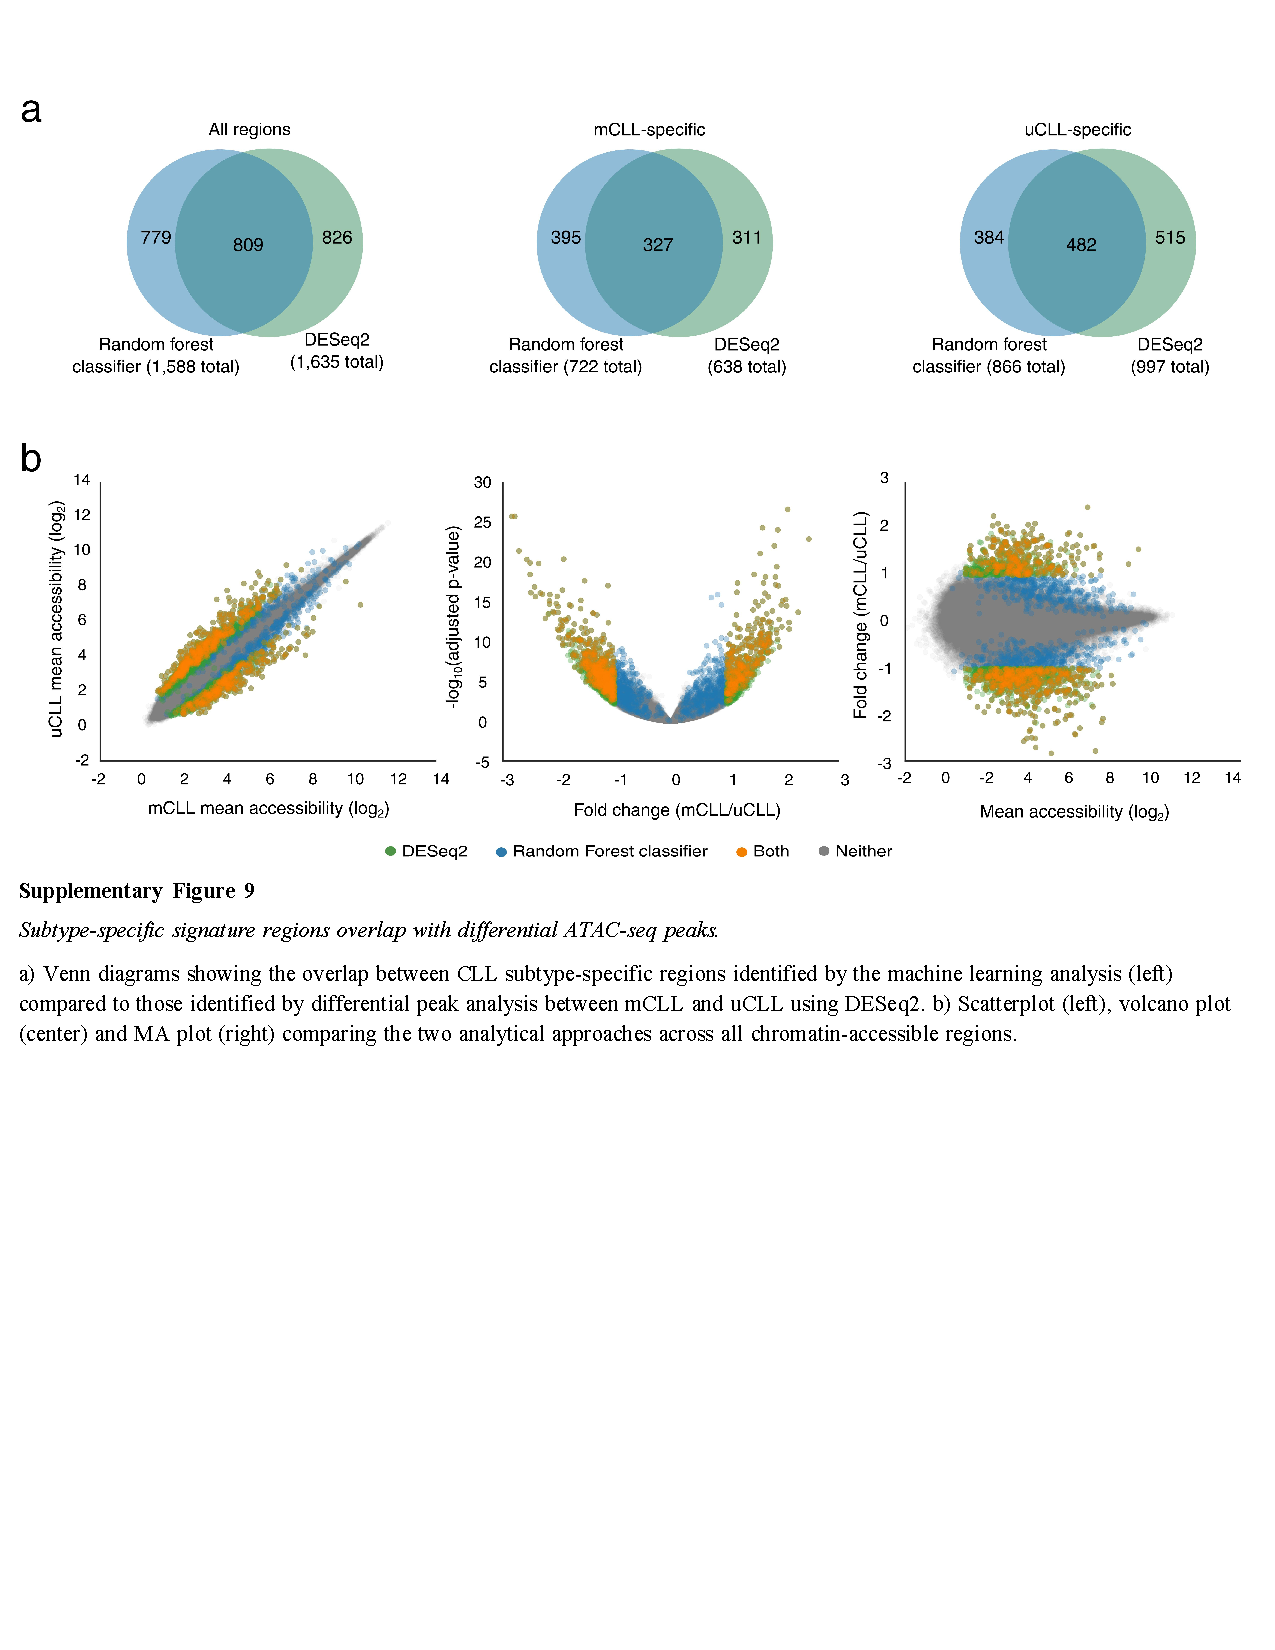
\includegraphics[width=1.000\hsize]{figures/Supplementary_Information_09.pdf}
\end{figure}
\clearpage

\begin{figure}
\centering
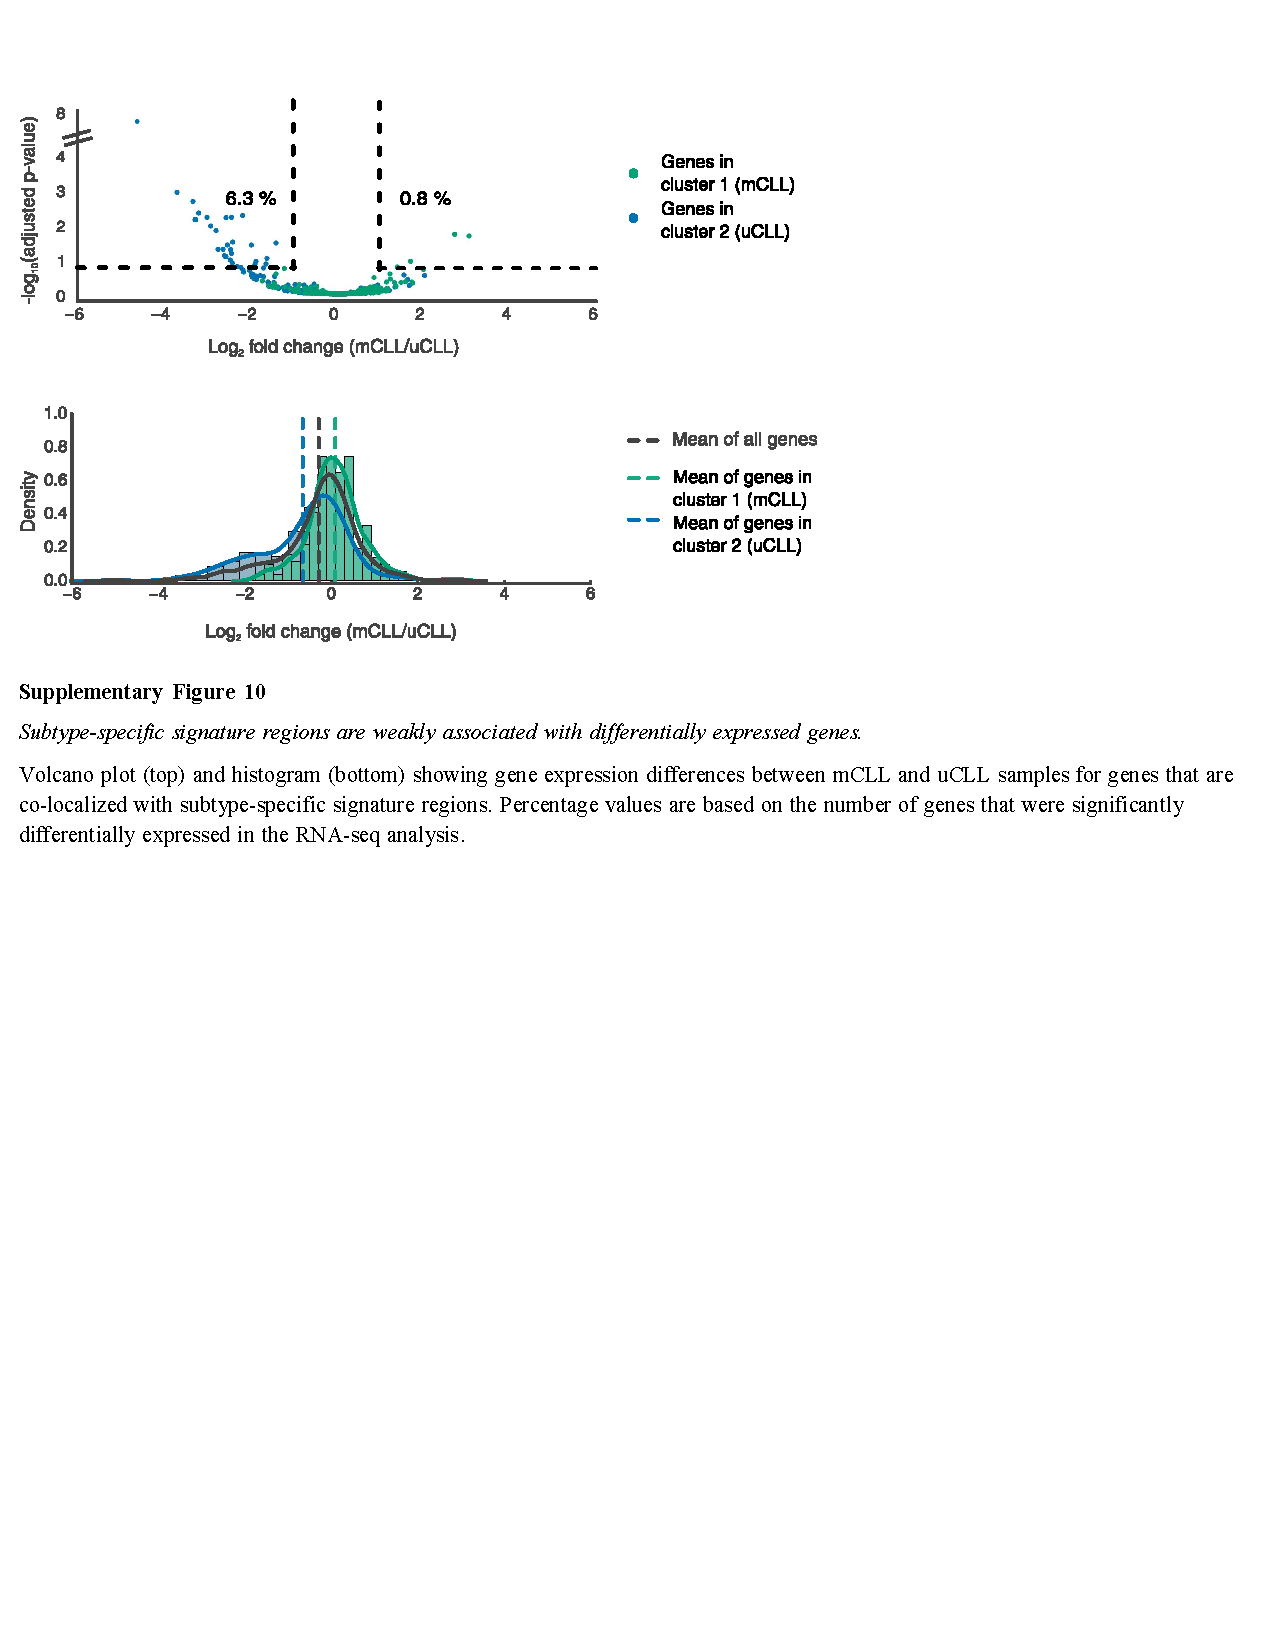
\includegraphics[width=1.000\hsize]{figures/Supplementary_Information_10.pdf}
\end{figure}
\clearpage

\begin{figure}
\centering
\includegraphics[width=1.000\hsize]{figures/Supplementary_Information_11.pdf}
\end{figure}
\clearpage

\begin{figure}
\centering
\includegraphics[width=1.000\hsize]{figures/Supplementary_Information_12.pdf}
\end{figure}
\clearpage

\begin{figure}
\centering
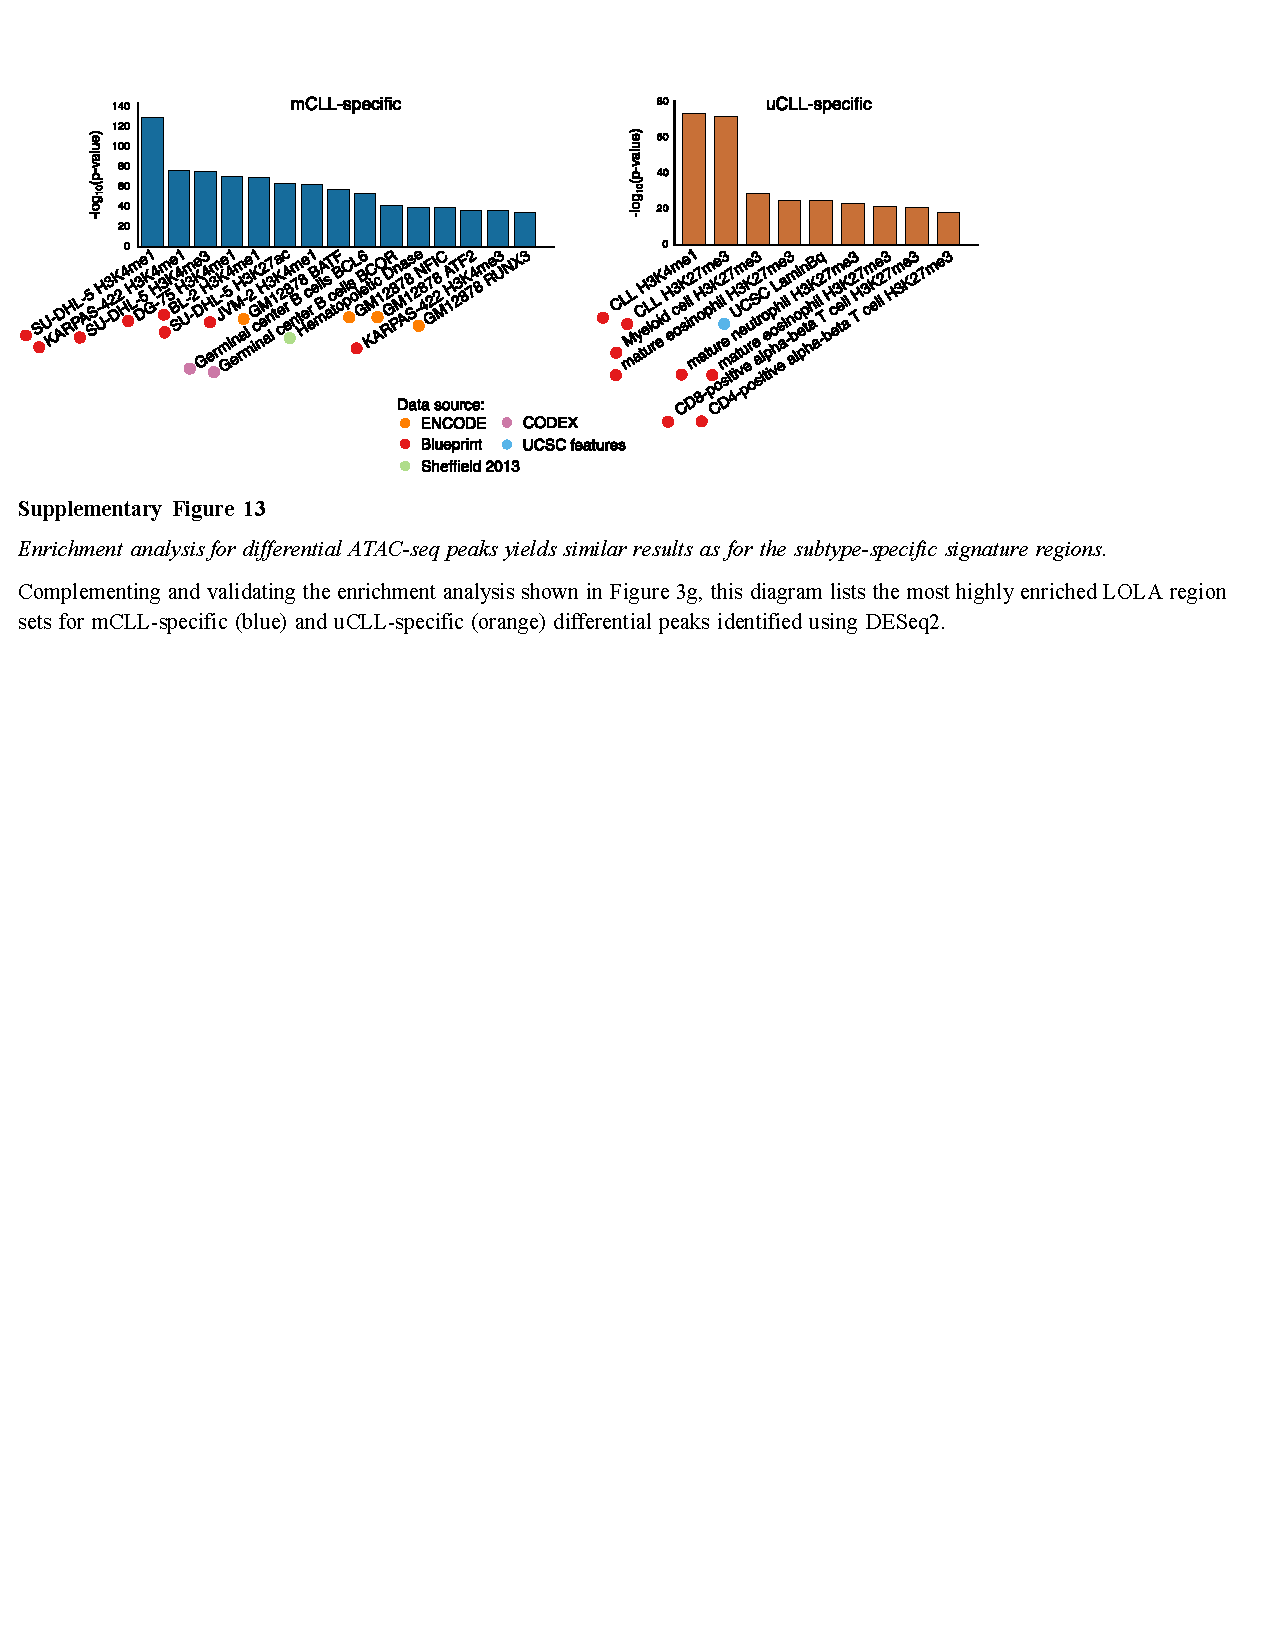
\includegraphics[width=1.000\hsize]{figures/Supplementary_Information_13.pdf}
\end{figure}
\clearpage

\begin{figure}
\centering
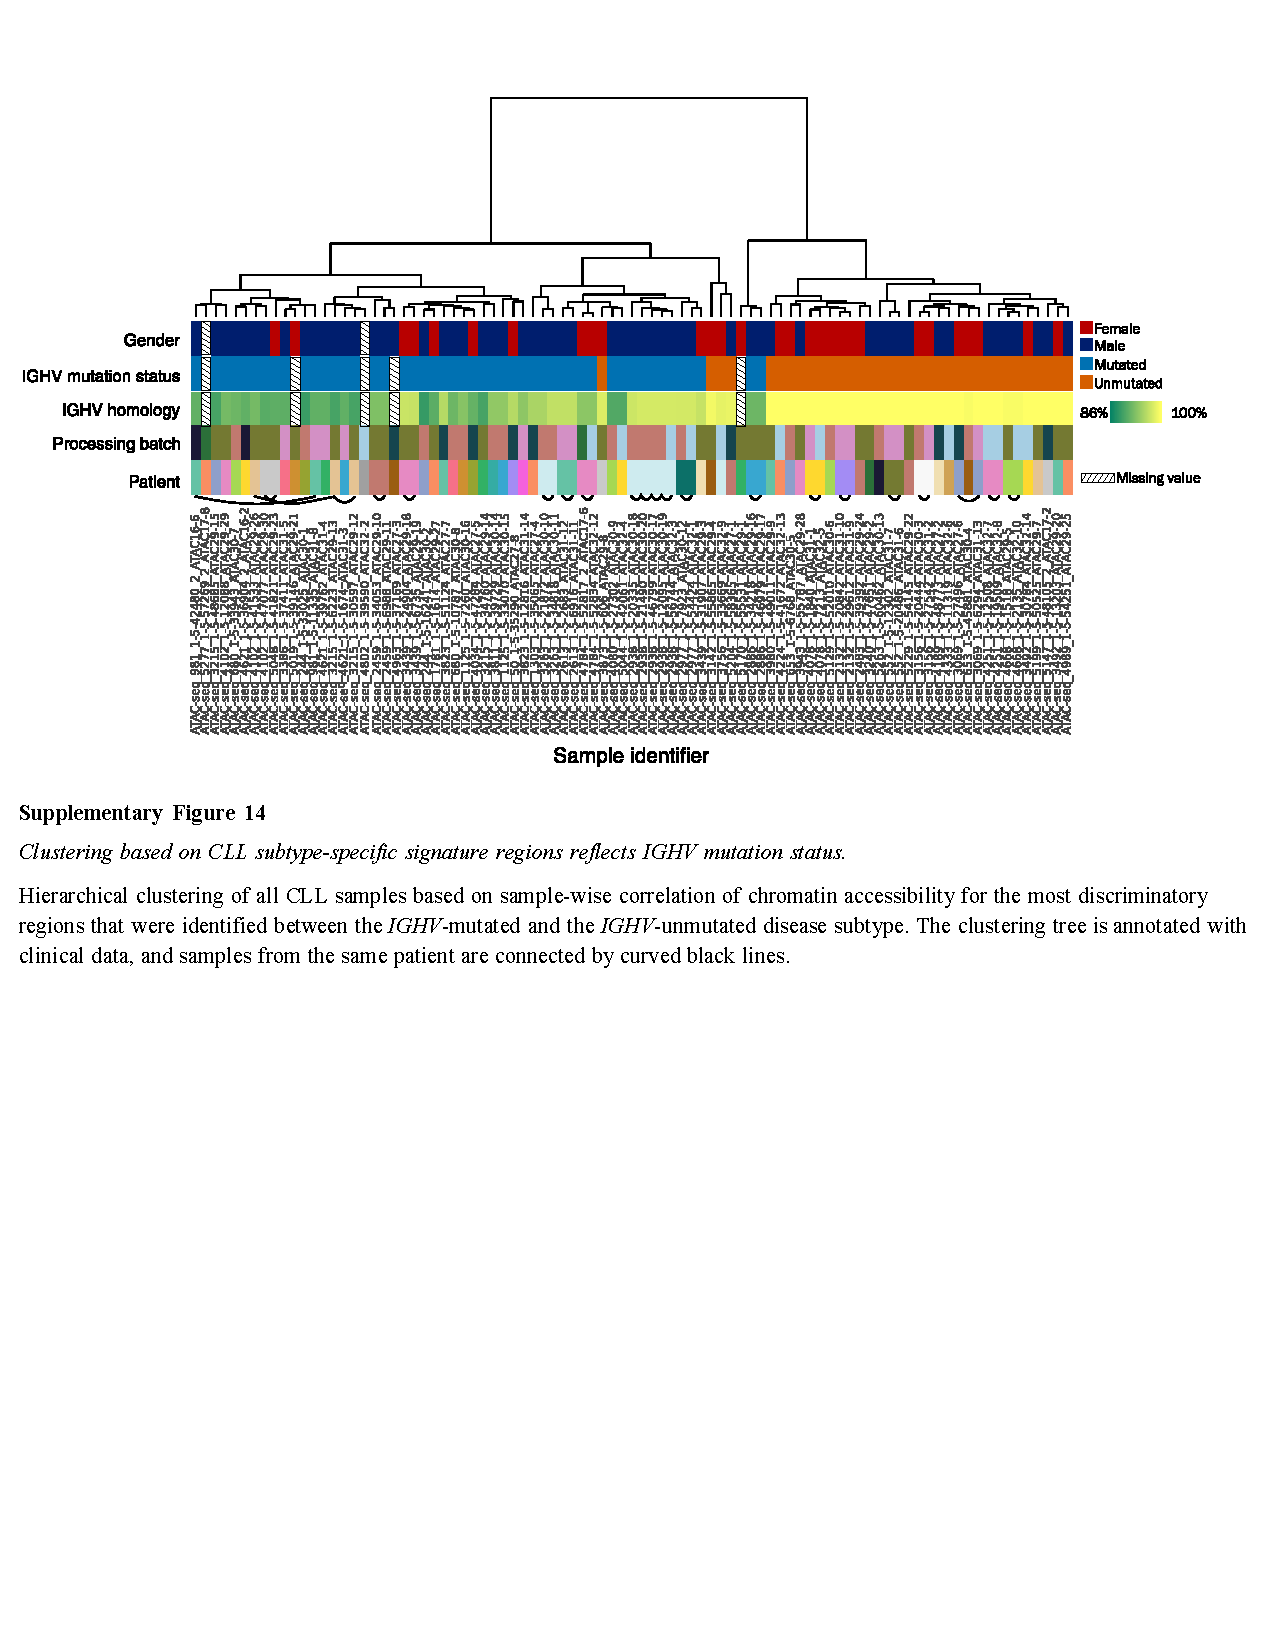
\includegraphics[width=1.000\hsize]{figures/Supplementary_Information_14.pdf}
\end{figure}
\clearpage

\begin{figure}
\centering
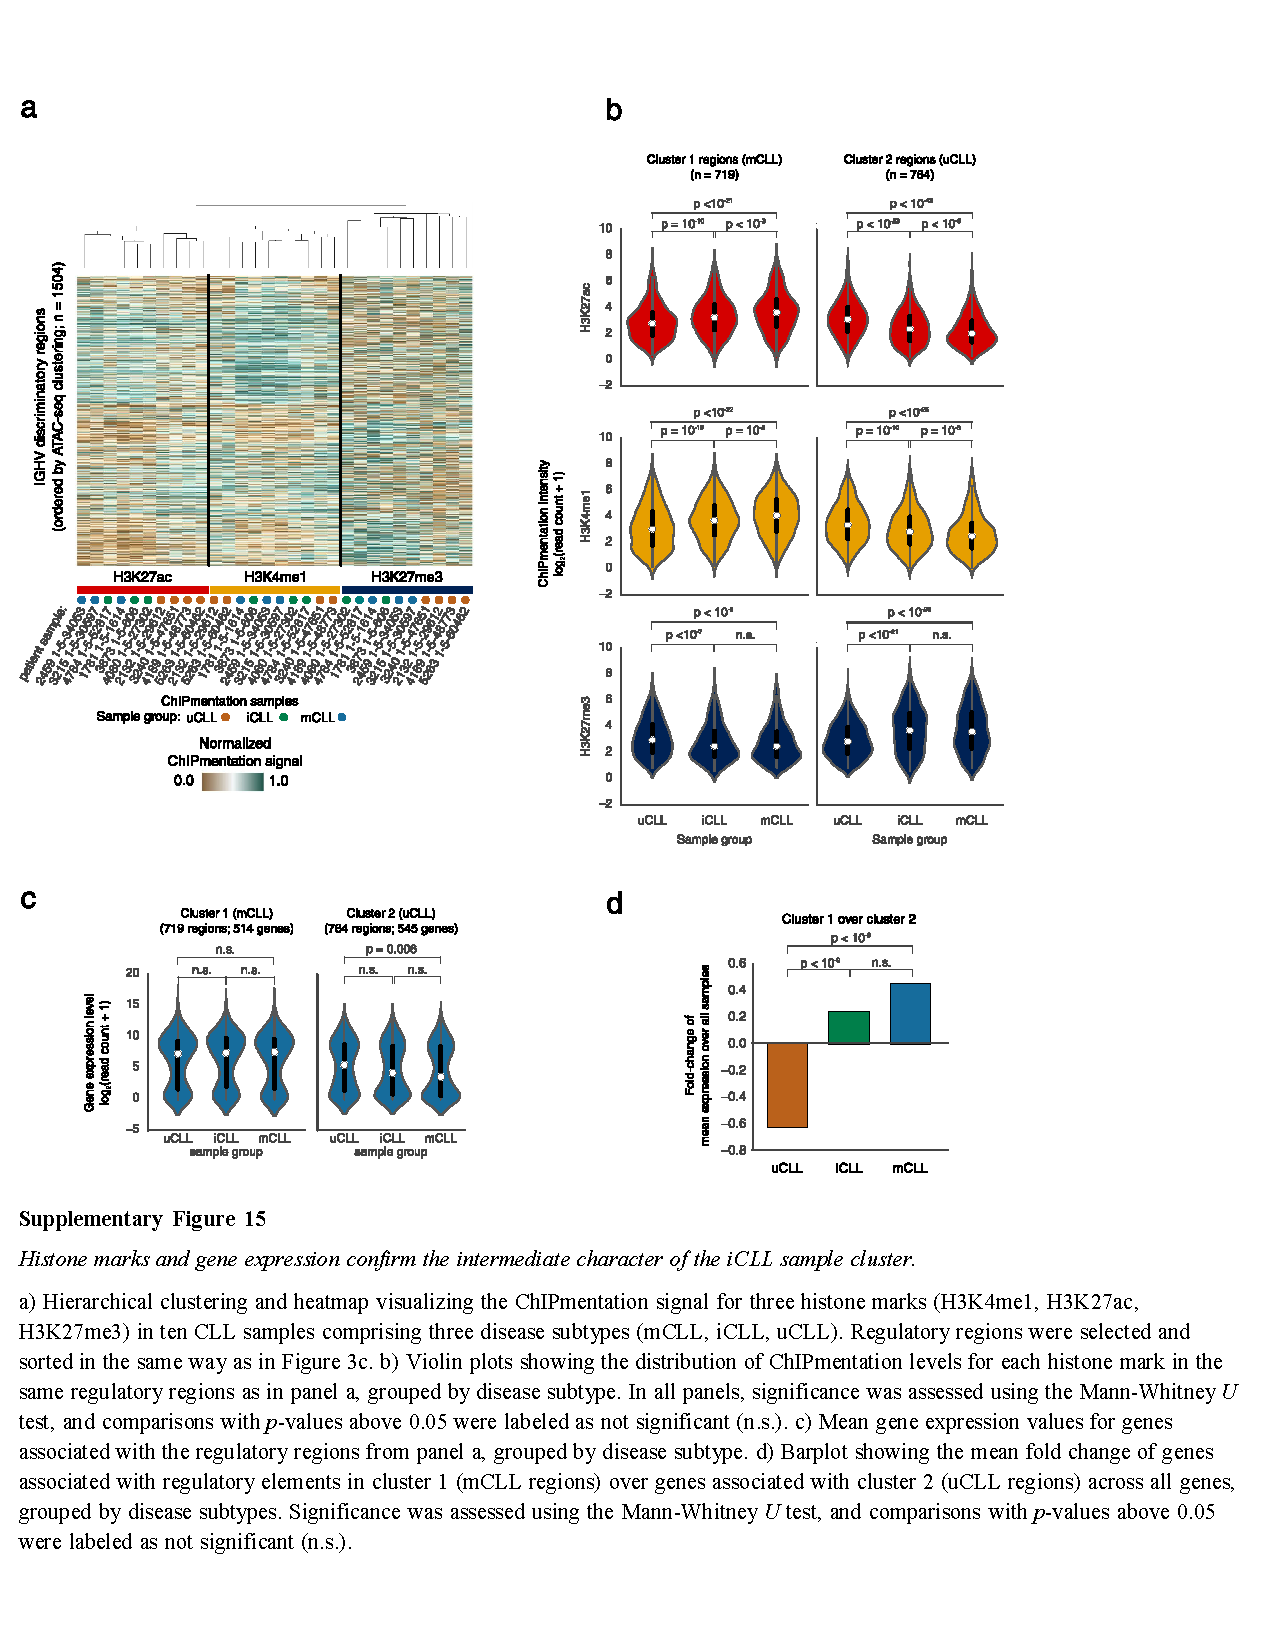
\includegraphics[width=1.000\hsize]{figures/Supplementary_Information_15.pdf}
\end{figure}
\clearpage

\begin{figure}
\centering
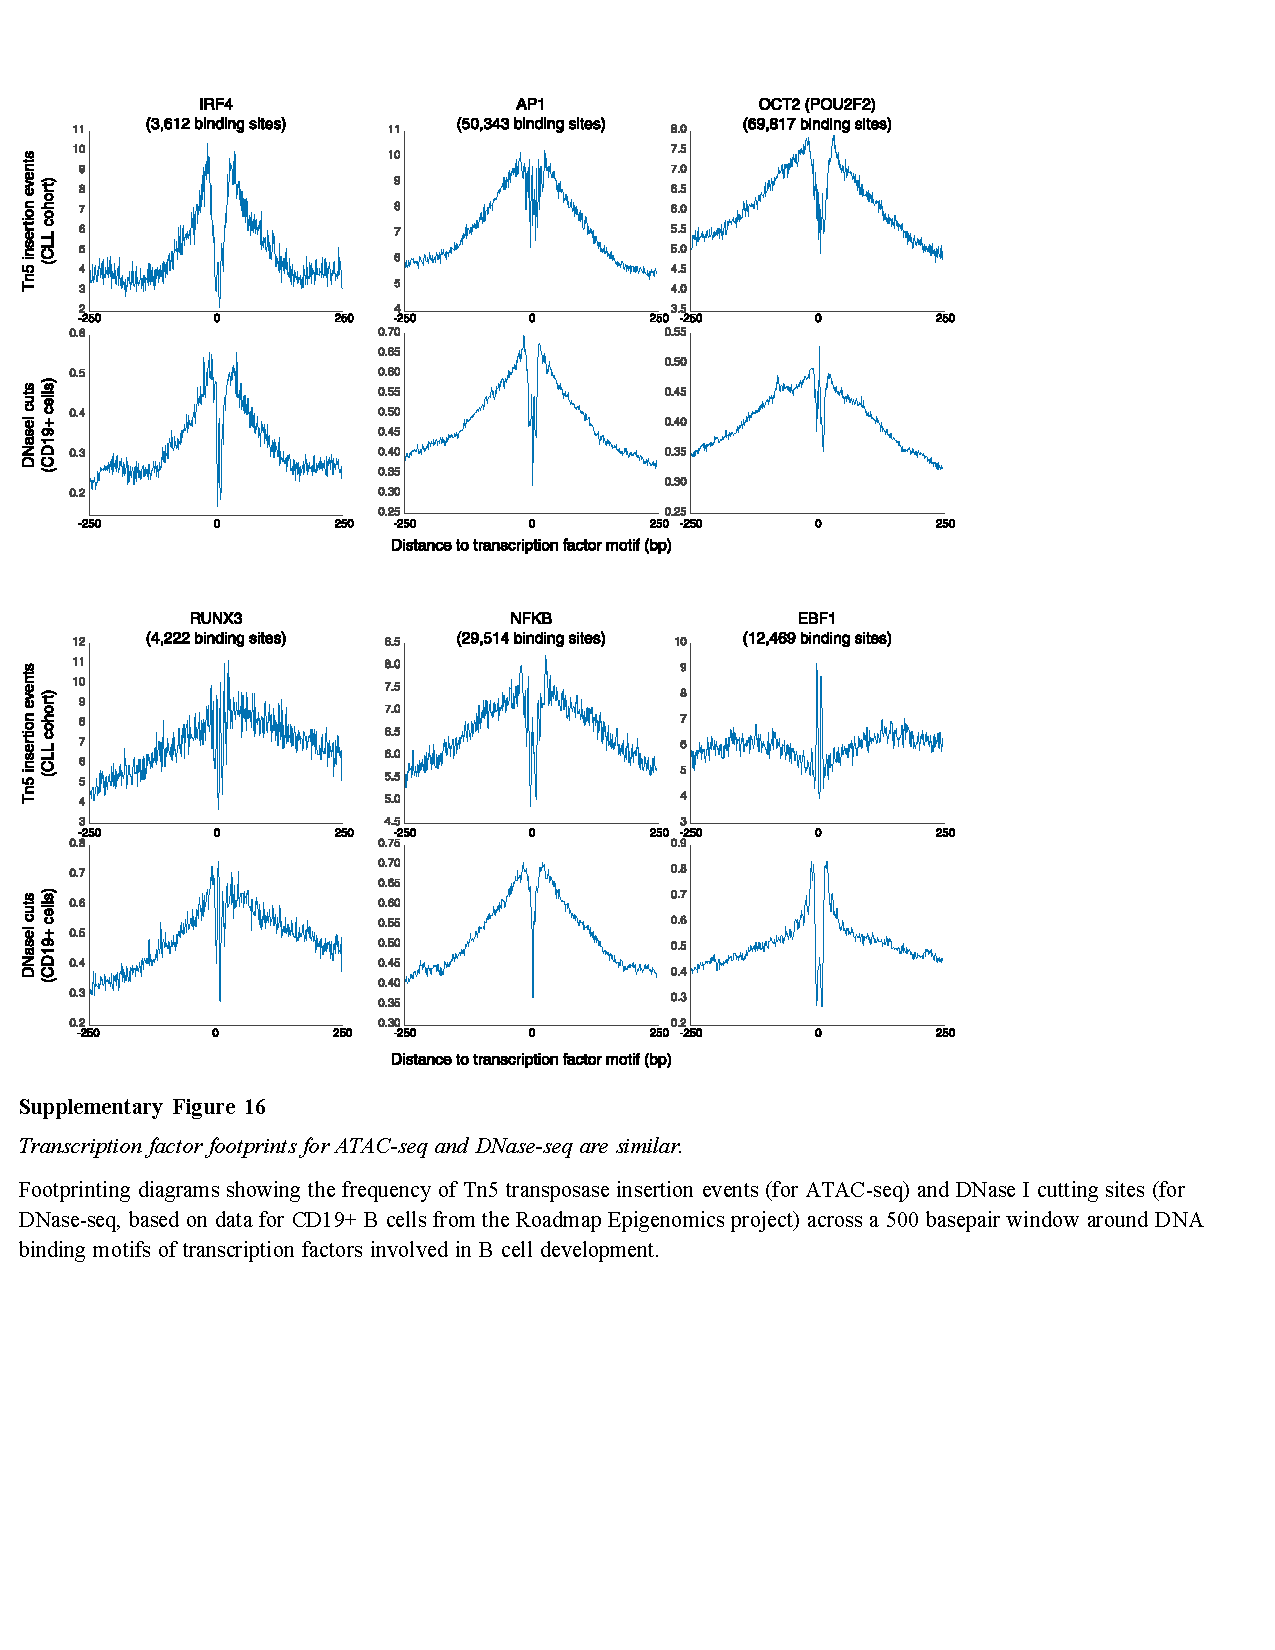
\includegraphics[width=1.000\hsize]{figures/Supplementary_Information_16.pdf}
\end{figure}
\clearpage

\begin{figure}
\centering
\includegraphics[width=1.000\hsize]{figures/Supplementary_Information_17.pdf}
\end{figure}
\clearpage

\begin{figure}
\centering
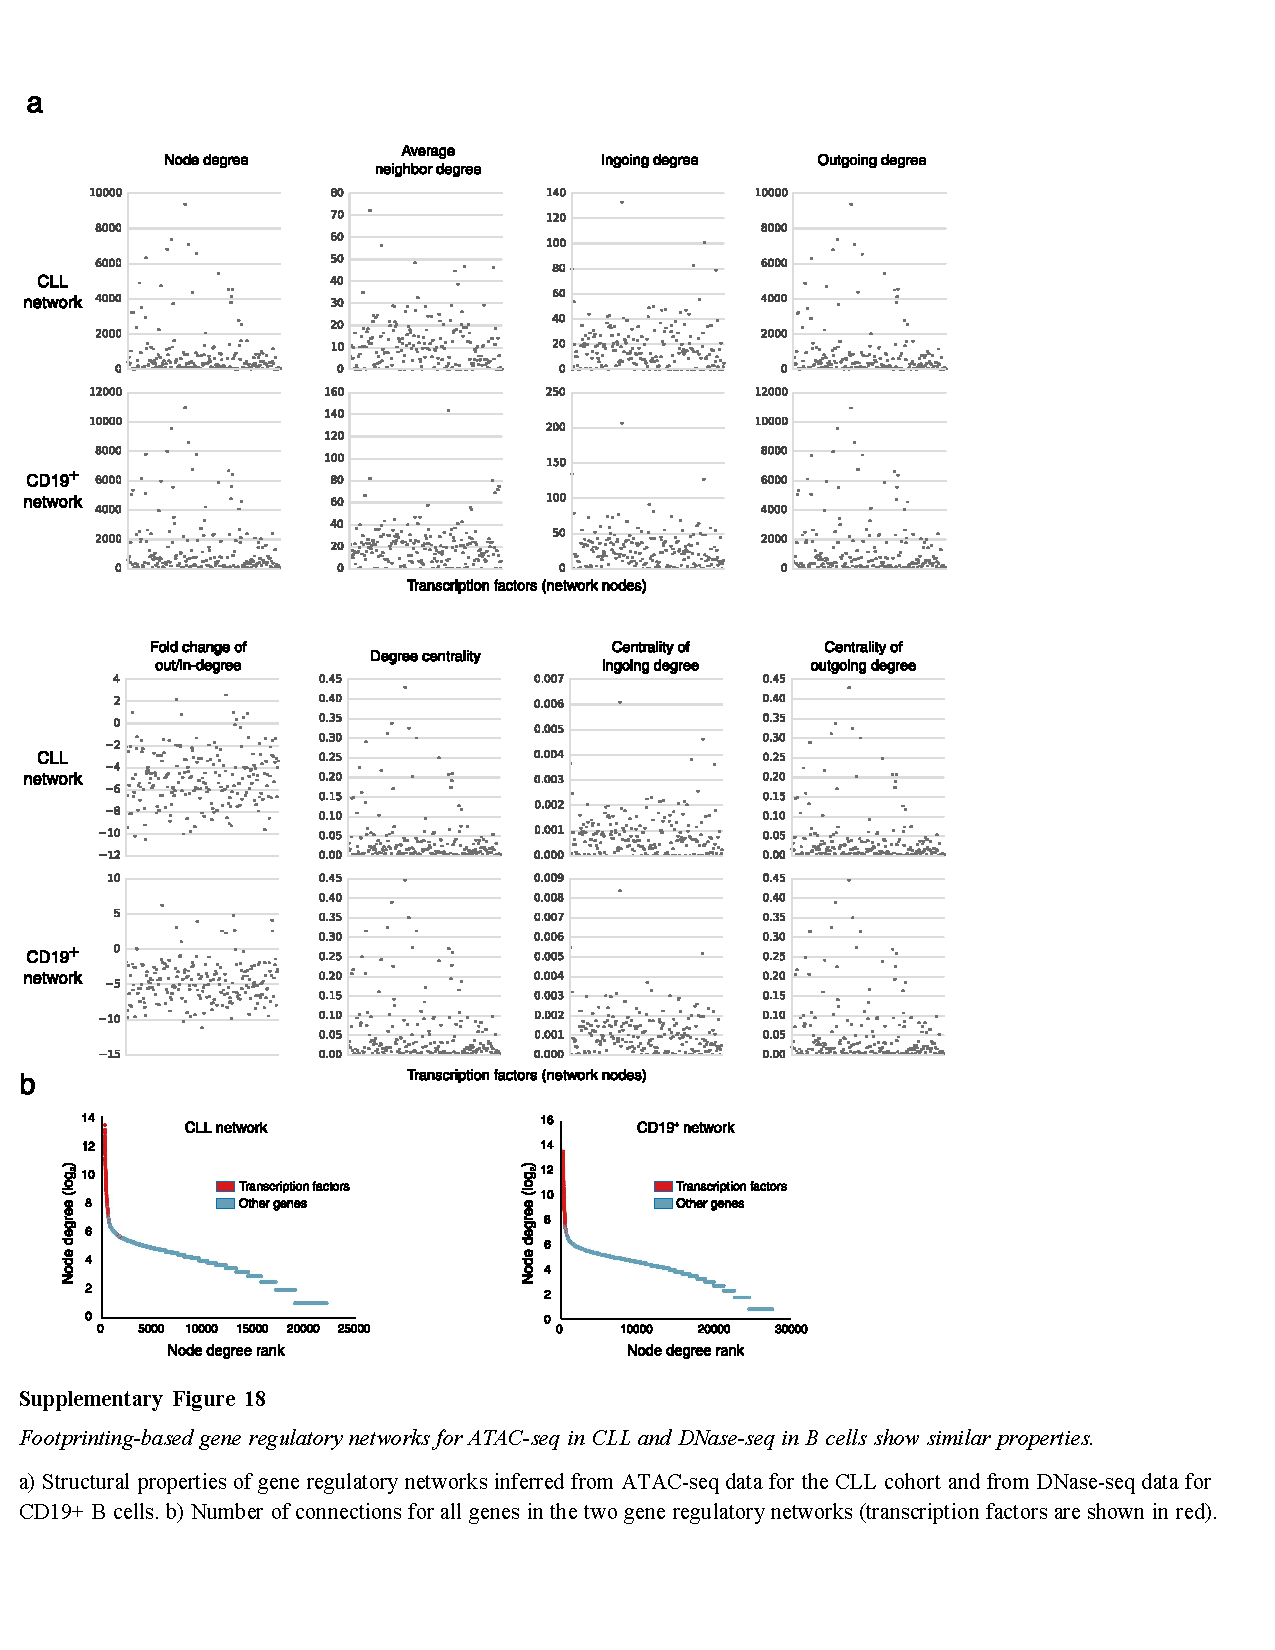
\includegraphics[width=1.000\hsize]{figures/Supplementary_Information_18.pdf}
\end{figure}
\clearpage

\begin{figure}
\centering
\includegraphics[width=1.000\hsize]{figures/Supplementary_Information_19.pdf}
\end{figure}
\clearpage

\begin{figure}
\centering
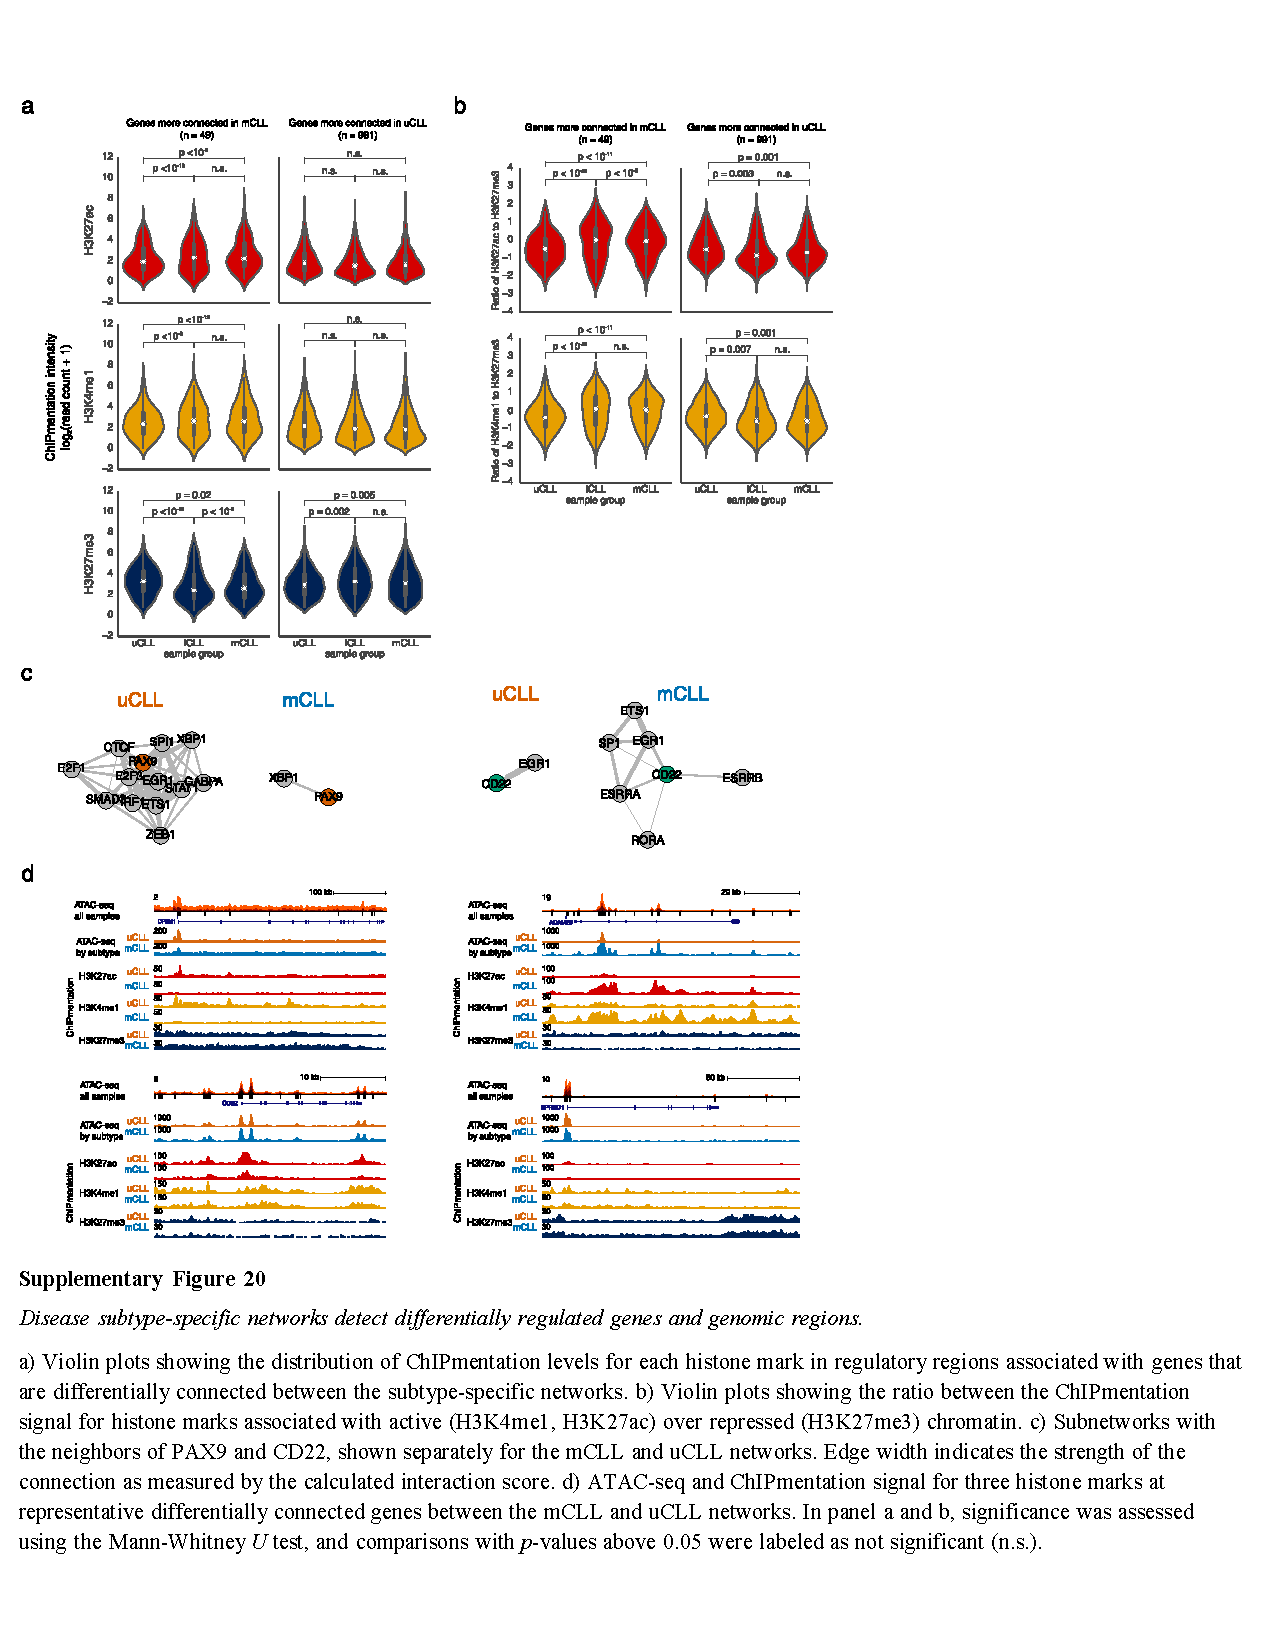
\includegraphics[width=1.000\hsize]{figures/Supplementary_Information_20.pdf}
\end{figure}
\clearpage

\renewcommand\refname{References}
\bibliography{/home/afr/Documents/library}


\end{document}

